\documentclass[12pt,]{article}
\usepackage[]{mathpazo}
\usepackage{amssymb,amsmath}
\usepackage{ifxetex,ifluatex}
\usepackage{fixltx2e} % provides \textsubscript
\ifnum 0\ifxetex 1\fi\ifluatex 1\fi=0 % if pdftex
  \usepackage[T1]{fontenc}
  \usepackage[utf8]{inputenc}
\else % if luatex or xelatex
  \ifxetex
    \usepackage{mathspec}
  \else
    \usepackage{fontspec}
  \fi
  \defaultfontfeatures{Ligatures=TeX,Scale=MatchLowercase}
\fi
% use upquote if available, for straight quotes in verbatim environments
\IfFileExists{upquote.sty}{\usepackage{upquote}}{}
% use microtype if available
\IfFileExists{microtype.sty}{%
\usepackage{microtype}
\UseMicrotypeSet[protrusion]{basicmath} % disable protrusion for tt fonts
}{}
\usepackage[margin=0.5in]{geometry}
\usepackage{hyperref}
\hypersetup{unicode=true,
            pdfborder={0 0 0},
            breaklinks=true}
\urlstyle{same}  % don't use monospace font for urls
\usepackage{color}
\usepackage{fancyvrb}
\newcommand{\VerbBar}{|}
\newcommand{\VERB}{\Verb[commandchars=\\\{\}]}
\DefineVerbatimEnvironment{Highlighting}{Verbatim}{commandchars=\\\{\}}
% Add ',fontsize=\small' for more characters per line
\usepackage{framed}
\definecolor{shadecolor}{RGB}{248,248,248}
\newenvironment{Shaded}{\begin{snugshade}}{\end{snugshade}}
\newcommand{\AlertTok}[1]{\textcolor[rgb]{0.94,0.16,0.16}{#1}}
\newcommand{\AnnotationTok}[1]{\textcolor[rgb]{0.56,0.35,0.01}{\textbf{\textit{#1}}}}
\newcommand{\AttributeTok}[1]{\textcolor[rgb]{0.77,0.63,0.00}{#1}}
\newcommand{\BaseNTok}[1]{\textcolor[rgb]{0.00,0.00,0.81}{#1}}
\newcommand{\BuiltInTok}[1]{#1}
\newcommand{\CharTok}[1]{\textcolor[rgb]{0.31,0.60,0.02}{#1}}
\newcommand{\CommentTok}[1]{\textcolor[rgb]{0.56,0.35,0.01}{\textit{#1}}}
\newcommand{\CommentVarTok}[1]{\textcolor[rgb]{0.56,0.35,0.01}{\textbf{\textit{#1}}}}
\newcommand{\ConstantTok}[1]{\textcolor[rgb]{0.00,0.00,0.00}{#1}}
\newcommand{\ControlFlowTok}[1]{\textcolor[rgb]{0.13,0.29,0.53}{\textbf{#1}}}
\newcommand{\DataTypeTok}[1]{\textcolor[rgb]{0.13,0.29,0.53}{#1}}
\newcommand{\DecValTok}[1]{\textcolor[rgb]{0.00,0.00,0.81}{#1}}
\newcommand{\DocumentationTok}[1]{\textcolor[rgb]{0.56,0.35,0.01}{\textbf{\textit{#1}}}}
\newcommand{\ErrorTok}[1]{\textcolor[rgb]{0.64,0.00,0.00}{\textbf{#1}}}
\newcommand{\ExtensionTok}[1]{#1}
\newcommand{\FloatTok}[1]{\textcolor[rgb]{0.00,0.00,0.81}{#1}}
\newcommand{\FunctionTok}[1]{\textcolor[rgb]{0.00,0.00,0.00}{#1}}
\newcommand{\ImportTok}[1]{#1}
\newcommand{\InformationTok}[1]{\textcolor[rgb]{0.56,0.35,0.01}{\textbf{\textit{#1}}}}
\newcommand{\KeywordTok}[1]{\textcolor[rgb]{0.13,0.29,0.53}{\textbf{#1}}}
\newcommand{\NormalTok}[1]{#1}
\newcommand{\OperatorTok}[1]{\textcolor[rgb]{0.81,0.36,0.00}{\textbf{#1}}}
\newcommand{\OtherTok}[1]{\textcolor[rgb]{0.56,0.35,0.01}{#1}}
\newcommand{\PreprocessorTok}[1]{\textcolor[rgb]{0.56,0.35,0.01}{\textit{#1}}}
\newcommand{\RegionMarkerTok}[1]{#1}
\newcommand{\SpecialCharTok}[1]{\textcolor[rgb]{0.00,0.00,0.00}{#1}}
\newcommand{\SpecialStringTok}[1]{\textcolor[rgb]{0.31,0.60,0.02}{#1}}
\newcommand{\StringTok}[1]{\textcolor[rgb]{0.31,0.60,0.02}{#1}}
\newcommand{\VariableTok}[1]{\textcolor[rgb]{0.00,0.00,0.00}{#1}}
\newcommand{\VerbatimStringTok}[1]{\textcolor[rgb]{0.31,0.60,0.02}{#1}}
\newcommand{\WarningTok}[1]{\textcolor[rgb]{0.56,0.35,0.01}{\textbf{\textit{#1}}}}
\usepackage{longtable,booktabs}
\usepackage{graphicx,grffile}
\makeatletter
\def\maxwidth{\ifdim\Gin@nat@width>\linewidth\linewidth\else\Gin@nat@width\fi}
\def\maxheight{\ifdim\Gin@nat@height>\textheight\textheight\else\Gin@nat@height\fi}
\makeatother
% Scale images if necessary, so that they will not overflow the page
% margins by default, and it is still possible to overwrite the defaults
% using explicit options in \includegraphics[width, height, ...]{}
\setkeys{Gin}{width=\maxwidth,height=\maxheight,keepaspectratio}
\IfFileExists{parskip.sty}{%
\usepackage{parskip}
}{% else
\setlength{\parindent}{0pt}
\setlength{\parskip}{6pt plus 2pt minus 1pt}
}
\setlength{\emergencystretch}{3em}  % prevent overfull lines
\providecommand{\tightlist}{%
  \setlength{\itemsep}{0pt}\setlength{\parskip}{0pt}}
\setcounter{secnumdepth}{0}
% Redefines (sub)paragraphs to behave more like sections
\ifx\paragraph\undefined\else
\let\oldparagraph\paragraph
\renewcommand{\paragraph}[1]{\oldparagraph{#1}\mbox{}}
\fi
\ifx\subparagraph\undefined\else
\let\oldsubparagraph\subparagraph
\renewcommand{\subparagraph}[1]{\oldsubparagraph{#1}\mbox{}}
\fi

%%% Use protect on footnotes to avoid problems with footnotes in titles
\let\rmarkdownfootnote\footnote%
\def\footnote{\protect\rmarkdownfootnote}

%%% Change title format to be more compact
\usepackage{titling}

% Create subtitle command for use in maketitle
\providecommand{\subtitle}[1]{
  \posttitle{
    \begin{center}\large#1\end{center}
    }
}

\setlength{\droptitle}{-2em}

  \title{}
    \pretitle{\vspace{\droptitle}}
  \posttitle{}
    \author{}
    \preauthor{}\postauthor{}
    \date{}
    \predate{}\postdate{}
  
\usepackage{booktabs}
\usepackage{longtable}
\usepackage{array}
\usepackage{multirow}
\usepackage{wrapfig}
\usepackage{float}
\usepackage{colortbl}
\usepackage{pdflscape}
\usepackage{tabu}
\usepackage{threeparttable}
\usepackage{threeparttablex}
\usepackage[normalem]{ulem}
\usepackage{makecell}
\usepackage{xcolor}

\begin{document}

\hypertarget{question-1}{%
\subsubsection{Question 1}\label{question-1}}

\textcolor[rgb]{0.7,0.7,0.7}{A process engineer is testing the yield of a product manufactured on randomly selected three machines. Each machine can be operated at a large number of power settings and only two power settings are randomly selected for this study. Furthermore, a machine has only three stations on which the product is formed. An experiment is conducted in which each machine is tested at both power settings, and three observations on yield are taken from each station. The runs are made in random order.
Part of the ANOVA table computed for the above experiment incorrectly treating all main effects as fixed and all combinations of factors as crossed is given below.}

\begin{longtable}[]{@{}ll@{}}
\toprule
\begin{minipage}[b]{0.35\columnwidth}\raggedright
Source\strut
\end{minipage} & \begin{minipage}[b]{0.13\columnwidth}\raggedright
SS\strut
\end{minipage}\tabularnewline
\midrule
\endhead
\begin{minipage}[t]{0.35\columnwidth}\raggedright
Machine\strut
\end{minipage} & \begin{minipage}[t]{0.13\columnwidth}\raggedright
21.436\strut
\end{minipage}\tabularnewline
\begin{minipage}[t]{0.35\columnwidth}\raggedright
Power\strut
\end{minipage} & \begin{minipage}[t]{0.13\columnwidth}\raggedright
845.698\strut
\end{minipage}\tabularnewline
\begin{minipage}[t]{0.35\columnwidth}\raggedright
Station\strut
\end{minipage} & \begin{minipage}[t]{0.13\columnwidth}\raggedright
16.980\strut
\end{minipage}\tabularnewline
\begin{minipage}[t]{0.35\columnwidth}\raggedright
Machine × Power\strut
\end{minipage} & \begin{minipage}[t]{0.13\columnwidth}\raggedright
0.383\strut
\end{minipage}\tabularnewline
\begin{minipage}[t]{0.35\columnwidth}\raggedright
Machine × Station\strut
\end{minipage} & \begin{minipage}[t]{0.13\columnwidth}\raggedright
16.603\strut
\end{minipage}\tabularnewline
\begin{minipage}[t]{0.35\columnwidth}\raggedright
Power × Station\strut
\end{minipage} & \begin{minipage}[t]{0.13\columnwidth}\raggedright
16.303\strut
\end{minipage}\tabularnewline
\begin{minipage}[t]{0.35\columnwidth}\raggedright
Machine × Power × Station\strut
\end{minipage} & \begin{minipage}[t]{0.13\columnwidth}\raggedright
12.905\strut
\end{minipage}\tabularnewline
\begin{minipage}[t]{0.35\columnwidth}\raggedright
Error\strut
\end{minipage} & \begin{minipage}[t]{0.13\columnwidth}\raggedright
61.760\strut
\end{minipage}\tabularnewline
\begin{minipage}[t]{0.35\columnwidth}\raggedright
Total\strut
\end{minipage} & \begin{minipage}[t]{0.13\columnwidth}\raggedright
992.068\strut
\end{minipage}\tabularnewline
\bottomrule
\end{longtable}

The model of the nested \& crossed Design is

\[y_{ijkl}=\mu+\tau_i+\beta_{j}+\gamma_{k(i)}+(\tau\beta)_{ij}+(\beta\gamma)_{jk(i)}+\varepsilon_{l(ijk)}\]

for \(i=1,2,3\) is the number of Machine being compared; \(j=1,2\) is
the number of Power being compared; \(k=1,2,3\) is the number of
stations; \(l=1,2,3\) is the number of replication;

\(\mu\) is the overall true mean response;

\(\tau_i\) is the random effect of \(i^{th}\) level of Machine;

\(\beta_{j}\) is the random effect of \(j^{th}\) level of Power;

\(\gamma_{k(i)}\) is the main fixed effect of \(k^{th}\) stations nested
in \(i^{th}\) level of Machine;

\((\tau\beta)_{ij}\) is the interaction effect of \(i^{th}\) level of
Machine and \(j^{th}\) level of Power;

\((\beta\gamma)_{jk(i)}\) is the interaction effect of \(j^{th}\) level
of Power and \(k^{th}\) stations nested in \(i^{th}\) level of Machine.

\(y_{ijkl}\) is response value for the \(l^{th}\) replication for
\(k^{th}\) stations nested in \(i^{th}\) level of Machine when
\(j^{th}\) level of Power is applied;

\(\varepsilon_{l(ijk)}\) is random error for the \(l^{th}\) replication
for \(k^{th}\) stations nested in \(i^{th}\) level of Machine when
\(j^{th}\) level of Power is applied.

Assumptions:

\begin{longtable}[]{@{}lll@{}}
\toprule
\begin{minipage}[b]{0.30\columnwidth}\raggedright
\(\varepsilon_{l(ijk)}\sim iid N(0,\sigma^2)\)\strut
\end{minipage} & \begin{minipage}[b]{0.30\columnwidth}\raggedright
\(\tau_{i}\sim iid N(0,\sigma_{\tau}^2)\)\strut
\end{minipage} & \begin{minipage}[b]{0.30\columnwidth}\raggedright
\(\beta_{j}\sim iid N(0,\sigma_{\beta}^2)\)\strut
\end{minipage}\tabularnewline
\midrule
\endhead
\begin{minipage}[t]{0.30\columnwidth}\raggedright
\(\sum_{k=1}^3\gamma_{k(i)}=0\)\strut
\end{minipage} & \begin{minipage}[t]{0.30\columnwidth}\raggedright
\((\tau\beta)_{ij}\sim iid N(0,\sigma_{\tau\beta}^2)\)\strut
\end{minipage} & \begin{minipage}[t]{0.30\columnwidth}\raggedright
\((\beta\gamma)_{jk(i)}\sim iid N(0,\frac{3-1}{3}\sigma_{\beta\gamma}^2)\)\strut
\end{minipage}\tabularnewline
\bottomrule
\end{longtable}

\(\varepsilon_{l(ijk)}\), \(\tau_{i}\), \(\beta_{j}\),
\((\tau\beta)_{ij}\), and \((\beta\gamma)_{jk(i)}\) are independent. For
restricted model, \(\sum_{k=1}^3(\beta\gamma)_{jk(i)}=0\)

\textcolor[rgb]{0.7,0.7,0.7}{Produce the corrected ANOVA table with Source, df, SS, MS, EMS, F value along with numerator and denominator df, and p value for each test.}

\begin{longtable}[]{@{}lllllllll@{}}
\toprule
\begin{minipage}[b]{0.06\columnwidth}\raggedright
source\strut
\end{minipage} & \begin{minipage}[b]{0.03\columnwidth}\raggedright
i(r)\strut
\end{minipage} & \begin{minipage}[b]{0.03\columnwidth}\raggedright
j(r)\strut
\end{minipage} & \begin{minipage}[b]{0.03\columnwidth}\raggedright
k(f)\strut
\end{minipage} & \begin{minipage}[b]{0.03\columnwidth}\raggedright
l(r)\strut
\end{minipage} & \begin{minipage}[b]{0.12\columnwidth}\raggedright
df\strut
\end{minipage} & \begin{minipage}[b]{0.15\columnwidth}\raggedright
SS\strut
\end{minipage} & \begin{minipage}[b]{0.21\columnwidth}\raggedright
EMS\strut
\end{minipage} & \begin{minipage}[b]{0.09\columnwidth}\raggedright
F\strut
\end{minipage}\tabularnewline
\midrule
\endhead
\begin{minipage}[t]{0.06\columnwidth}\raggedright
A\strut
\end{minipage} & \begin{minipage}[t]{0.03\columnwidth}\raggedright
1\strut
\end{minipage} & \begin{minipage}[t]{0.03\columnwidth}\raggedright
b\strut
\end{minipage} & \begin{minipage}[t]{0.03\columnwidth}\raggedright
c\strut
\end{minipage} & \begin{minipage}[t]{0.03\columnwidth}\raggedright
n\strut
\end{minipage} & \begin{minipage}[t]{0.12\columnwidth}\raggedright
a-1\strut
\end{minipage} & \begin{minipage}[t]{0.15\columnwidth}\raggedright
\(SS_A\)\strut
\end{minipage} & \begin{minipage}[t]{0.21\columnwidth}\raggedright
\(\sigma^2+cn\sigma^2_{\tau\beta}+bcn\sigma^2_{\tau_{i}}\)\strut
\end{minipage} & \begin{minipage}[t]{0.09\columnwidth}\raggedright
\(\frac{MS_{A}}{MS_{AB}}\)\strut
\end{minipage}\tabularnewline
\begin{minipage}[t]{0.06\columnwidth}\raggedright
\(\tau_{i}\)\strut
\end{minipage} & \begin{minipage}[t]{0.03\columnwidth}\raggedright
\strut
\end{minipage} & \begin{minipage}[t]{0.03\columnwidth}\raggedright
2\strut
\end{minipage} & \begin{minipage}[t]{0.03\columnwidth}\raggedright
3\strut
\end{minipage} & \begin{minipage}[t]{0.03\columnwidth}\raggedright
3\strut
\end{minipage} & \begin{minipage}[t]{0.12\columnwidth}\raggedright
3-1\strut
\end{minipage} & \begin{minipage}[t]{0.15\columnwidth}\raggedright
21.436\strut
\end{minipage} & \begin{minipage}[t]{0.21\columnwidth}\raggedright
\(\sigma^2+9\sigma^2_{\tau\beta}+18\sigma^2_{\tau_{i}}\)\strut
\end{minipage} & \begin{minipage}[t]{0.09\columnwidth}\raggedright
\(df_{2,2}\)\strut
\end{minipage}\tabularnewline
\begin{minipage}[t]{0.06\columnwidth}\raggedright
(r)\strut
\end{minipage} & \begin{minipage}[t]{0.03\columnwidth}\raggedright
\strut
\end{minipage} & \begin{minipage}[t]{0.03\columnwidth}\raggedright
\strut
\end{minipage} & \begin{minipage}[t]{0.03\columnwidth}\raggedright
\strut
\end{minipage} & \begin{minipage}[t]{0.03\columnwidth}\raggedright
\strut
\end{minipage} & \begin{minipage}[t]{0.12\columnwidth}\raggedright
\strut
\end{minipage} & \begin{minipage}[t]{0.15\columnwidth}\raggedright
\strut
\end{minipage} & \begin{minipage}[t]{0.21\columnwidth}\raggedright
\strut
\end{minipage} & \begin{minipage}[t]{0.09\columnwidth}\raggedright
\strut
\end{minipage}\tabularnewline
\begin{minipage}[t]{0.06\columnwidth}\raggedright
B\strut
\end{minipage} & \begin{minipage}[t]{0.03\columnwidth}\raggedright
a\strut
\end{minipage} & \begin{minipage}[t]{0.03\columnwidth}\raggedright
1\strut
\end{minipage} & \begin{minipage}[t]{0.03\columnwidth}\raggedright
c\strut
\end{minipage} & \begin{minipage}[t]{0.03\columnwidth}\raggedright
n\strut
\end{minipage} & \begin{minipage}[t]{0.12\columnwidth}\raggedright
b-1\strut
\end{minipage} & \begin{minipage}[t]{0.15\columnwidth}\raggedright
\(SS_B\)\strut
\end{minipage} & \begin{minipage}[t]{0.21\columnwidth}\raggedright
\(\sigma^2+cn\sigma^2_{\beta\gamma}+acn\sigma^2_{\tau\beta}\)\strut
\end{minipage} & \begin{minipage}[t]{0.09\columnwidth}\raggedright
\(\frac{MS_{B}}{MS_{AB}}\)\strut
\end{minipage}\tabularnewline
\begin{minipage}[t]{0.06\columnwidth}\raggedright
\(\beta_{j}\)\strut
\end{minipage} & \begin{minipage}[t]{0.03\columnwidth}\raggedright
3\strut
\end{minipage} & \begin{minipage}[t]{0.03\columnwidth}\raggedright
\strut
\end{minipage} & \begin{minipage}[t]{0.03\columnwidth}\raggedright
3\strut
\end{minipage} & \begin{minipage}[t]{0.03\columnwidth}\raggedright
3\strut
\end{minipage} & \begin{minipage}[t]{0.12\columnwidth}\raggedright
2-1\strut
\end{minipage} & \begin{minipage}[t]{0.15\columnwidth}\raggedright
845.698\strut
\end{minipage} & \begin{minipage}[t]{0.21\columnwidth}\raggedright
\(\sigma^2+9\sigma^2_{\beta\gamma}+27\sigma^2_{\tau\beta}\)\strut
\end{minipage} & \begin{minipage}[t]{0.09\columnwidth}\raggedright
\(df_{1,2}\)\strut
\end{minipage}\tabularnewline
\begin{minipage}[t]{0.06\columnwidth}\raggedright
(r)\strut
\end{minipage} & \begin{minipage}[t]{0.03\columnwidth}\raggedright
\strut
\end{minipage} & \begin{minipage}[t]{0.03\columnwidth}\raggedright
\strut
\end{minipage} & \begin{minipage}[t]{0.03\columnwidth}\raggedright
\strut
\end{minipage} & \begin{minipage}[t]{0.03\columnwidth}\raggedright
\strut
\end{minipage} & \begin{minipage}[t]{0.12\columnwidth}\raggedright
\strut
\end{minipage} & \begin{minipage}[t]{0.15\columnwidth}\raggedright
\strut
\end{minipage} & \begin{minipage}[t]{0.21\columnwidth}\raggedright
\strut
\end{minipage} & \begin{minipage}[t]{0.09\columnwidth}\raggedright
\strut
\end{minipage}\tabularnewline
\begin{minipage}[t]{0.06\columnwidth}\raggedright
C(A)\strut
\end{minipage} & \begin{minipage}[t]{0.03\columnwidth}\raggedright
1\strut
\end{minipage} & \begin{minipage}[t]{0.03\columnwidth}\raggedright
b\strut
\end{minipage} & \begin{minipage}[t]{0.03\columnwidth}\raggedright
0\strut
\end{minipage} & \begin{minipage}[t]{0.03\columnwidth}\raggedright
n\strut
\end{minipage} & \begin{minipage}[t]{0.12\columnwidth}\raggedright
a(c-1)\strut
\end{minipage} & \begin{minipage}[t]{0.15\columnwidth}\raggedright
\(SS_C+SS_{AC}\)\strut
\end{minipage} & \begin{minipage}[t]{0.21\columnwidth}\raggedright
\(\sigma^2+n\sigma^2_{\beta\gamma}+\frac{bn\sum\limits_{k=1}^c\gamma_{k(i)}^2}{c-1}\)\strut
\end{minipage} & \begin{minipage}[t]{0.09\columnwidth}\raggedright
\(\frac{MS_{C(A)}}{MS_{BC(A)}}\)\strut
\end{minipage}\tabularnewline
\begin{minipage}[t]{0.06\columnwidth}\raggedright
\(\gamma_{k(i)}\)\strut
\end{minipage} & \begin{minipage}[t]{0.03\columnwidth}\raggedright
\strut
\end{minipage} & \begin{minipage}[t]{0.03\columnwidth}\raggedright
2\strut
\end{minipage} & \begin{minipage}[t]{0.03\columnwidth}\raggedright
\strut
\end{minipage} & \begin{minipage}[t]{0.03\columnwidth}\raggedright
3\strut
\end{minipage} & \begin{minipage}[t]{0.12\columnwidth}\raggedright
3(3-1)\strut
\end{minipage} & \begin{minipage}[t]{0.15\columnwidth}\raggedright
16.980+16.603\strut
\end{minipage} & \begin{minipage}[t]{0.21\columnwidth}\raggedright
\(\sigma^2+3\sigma^2_{\beta\gamma}+3\sum\limits_{k=1}^3\gamma_{k(i)}^2\)\strut
\end{minipage} & \begin{minipage}[t]{0.09\columnwidth}\raggedright
\(df_{6,6}\)\strut
\end{minipage}\tabularnewline
\begin{minipage}[t]{0.06\columnwidth}\raggedright
(f)\strut
\end{minipage} & \begin{minipage}[t]{0.03\columnwidth}\raggedright
\strut
\end{minipage} & \begin{minipage}[t]{0.03\columnwidth}\raggedright
\strut
\end{minipage} & \begin{minipage}[t]{0.03\columnwidth}\raggedright
\strut
\end{minipage} & \begin{minipage}[t]{0.03\columnwidth}\raggedright
\strut
\end{minipage} & \begin{minipage}[t]{0.12\columnwidth}\raggedright
\strut
\end{minipage} & \begin{minipage}[t]{0.15\columnwidth}\raggedright
\strut
\end{minipage} & \begin{minipage}[t]{0.21\columnwidth}\raggedright
\strut
\end{minipage} & \begin{minipage}[t]{0.09\columnwidth}\raggedright
\strut
\end{minipage}\tabularnewline
\begin{minipage}[t]{0.06\columnwidth}\raggedright
AB\strut
\end{minipage} & \begin{minipage}[t]{0.03\columnwidth}\raggedright
1\strut
\end{minipage} & \begin{minipage}[t]{0.03\columnwidth}\raggedright
1\strut
\end{minipage} & \begin{minipage}[t]{0.03\columnwidth}\raggedright
c\strut
\end{minipage} & \begin{minipage}[t]{0.03\columnwidth}\raggedright
n\strut
\end{minipage} & \begin{minipage}[t]{0.12\columnwidth}\raggedright
(a-1)(b-1)\strut
\end{minipage} & \begin{minipage}[t]{0.15\columnwidth}\raggedright
\(SS_{AB}\)\strut
\end{minipage} & \begin{minipage}[t]{0.21\columnwidth}\raggedright
\(\sigma^2+cn\sigma^2_{\tau\beta}\)\strut
\end{minipage} & \begin{minipage}[t]{0.09\columnwidth}\raggedright
\(\frac{MS_{AB}}{MS_{E}}\)\strut
\end{minipage}\tabularnewline
\begin{minipage}[t]{0.06\columnwidth}\raggedright
\((\tau\beta)_{ij}\)\strut
\end{minipage} & \begin{minipage}[t]{0.03\columnwidth}\raggedright
\strut
\end{minipage} & \begin{minipage}[t]{0.03\columnwidth}\raggedright
\strut
\end{minipage} & \begin{minipage}[t]{0.03\columnwidth}\raggedright
3\strut
\end{minipage} & \begin{minipage}[t]{0.03\columnwidth}\raggedright
3\strut
\end{minipage} & \begin{minipage}[t]{0.12\columnwidth}\raggedright
(3-1)(2-1)\strut
\end{minipage} & \begin{minipage}[t]{0.15\columnwidth}\raggedright
0.383\strut
\end{minipage} & \begin{minipage}[t]{0.21\columnwidth}\raggedright
\(\sigma^2+9\sigma^2_{\tau\beta}\)\strut
\end{minipage} & \begin{minipage}[t]{0.09\columnwidth}\raggedright
\(df_{2,36}\)\strut
\end{minipage}\tabularnewline
\begin{minipage}[t]{0.06\columnwidth}\raggedright
(r)\strut
\end{minipage} & \begin{minipage}[t]{0.03\columnwidth}\raggedright
\strut
\end{minipage} & \begin{minipage}[t]{0.03\columnwidth}\raggedright
\strut
\end{minipage} & \begin{minipage}[t]{0.03\columnwidth}\raggedright
\strut
\end{minipage} & \begin{minipage}[t]{0.03\columnwidth}\raggedright
\strut
\end{minipage} & \begin{minipage}[t]{0.12\columnwidth}\raggedright
\strut
\end{minipage} & \begin{minipage}[t]{0.15\columnwidth}\raggedright
\strut
\end{minipage} & \begin{minipage}[t]{0.21\columnwidth}\raggedright
\strut
\end{minipage} & \begin{minipage}[t]{0.09\columnwidth}\raggedright
\strut
\end{minipage}\tabularnewline
\begin{minipage}[t]{0.06\columnwidth}\raggedright
BC(A)\strut
\end{minipage} & \begin{minipage}[t]{0.03\columnwidth}\raggedright
1\strut
\end{minipage} & \begin{minipage}[t]{0.03\columnwidth}\raggedright
1\strut
\end{minipage} & \begin{minipage}[t]{0.03\columnwidth}\raggedright
0\strut
\end{minipage} & \begin{minipage}[t]{0.03\columnwidth}\raggedright
n\strut
\end{minipage} & \begin{minipage}[t]{0.12\columnwidth}\raggedright
a(b-1)(c-1)\strut
\end{minipage} & \begin{minipage}[t]{0.15\columnwidth}\raggedright
\(SS_{BC}+SS_{ABC}\)\strut
\end{minipage} & \begin{minipage}[t]{0.21\columnwidth}\raggedright
\(\sigma^2+n\sigma^2_{\beta\gamma}\)\strut
\end{minipage} & \begin{minipage}[t]{0.09\columnwidth}\raggedright
\(\frac{MS_{BC(A)}}{MS_{E}}\)\strut
\end{minipage}\tabularnewline
\begin{minipage}[t]{0.06\columnwidth}\raggedright
\((\beta\gamma)_{jk(i)}\)\strut
\end{minipage} & \begin{minipage}[t]{0.03\columnwidth}\raggedright
\strut
\end{minipage} & \begin{minipage}[t]{0.03\columnwidth}\raggedright
\strut
\end{minipage} & \begin{minipage}[t]{0.03\columnwidth}\raggedright
\strut
\end{minipage} & \begin{minipage}[t]{0.03\columnwidth}\raggedright
3\strut
\end{minipage} & \begin{minipage}[t]{0.12\columnwidth}\raggedright
3(2-1)(3-1)\strut
\end{minipage} & \begin{minipage}[t]{0.15\columnwidth}\raggedright
16.303+12.905\strut
\end{minipage} & \begin{minipage}[t]{0.21\columnwidth}\raggedright
\(\sigma^2+3\sigma^2_{\beta\gamma}\)\strut
\end{minipage} & \begin{minipage}[t]{0.09\columnwidth}\raggedright
\(df_{6,36}\)\strut
\end{minipage}\tabularnewline
\begin{minipage}[t]{0.06\columnwidth}\raggedright
(r)\strut
\end{minipage} & \begin{minipage}[t]{0.03\columnwidth}\raggedright
\strut
\end{minipage} & \begin{minipage}[t]{0.03\columnwidth}\raggedright
\strut
\end{minipage} & \begin{minipage}[t]{0.03\columnwidth}\raggedright
\strut
\end{minipage} & \begin{minipage}[t]{0.03\columnwidth}\raggedright
\strut
\end{minipage} & \begin{minipage}[t]{0.12\columnwidth}\raggedright
\strut
\end{minipage} & \begin{minipage}[t]{0.15\columnwidth}\raggedright
\strut
\end{minipage} & \begin{minipage}[t]{0.21\columnwidth}\raggedright
\strut
\end{minipage} & \begin{minipage}[t]{0.09\columnwidth}\raggedright
\strut
\end{minipage}\tabularnewline
\begin{minipage}[t]{0.06\columnwidth}\raggedright
Error\strut
\end{minipage} & \begin{minipage}[t]{0.03\columnwidth}\raggedright
1\strut
\end{minipage} & \begin{minipage}[t]{0.03\columnwidth}\raggedright
1\strut
\end{minipage} & \begin{minipage}[t]{0.03\columnwidth}\raggedright
1\strut
\end{minipage} & \begin{minipage}[t]{0.03\columnwidth}\raggedright
1\strut
\end{minipage} & \begin{minipage}[t]{0.12\columnwidth}\raggedright
abc(n-1)\strut
\end{minipage} & \begin{minipage}[t]{0.15\columnwidth}\raggedright
\(SS_{E}\)\strut
\end{minipage} & \begin{minipage}[t]{0.21\columnwidth}\raggedright
\(\sigma^2\)\strut
\end{minipage} & \begin{minipage}[t]{0.09\columnwidth}\raggedright
\strut
\end{minipage}\tabularnewline
\begin{minipage}[t]{0.06\columnwidth}\raggedright
(r)\strut
\end{minipage} & \begin{minipage}[t]{0.03\columnwidth}\raggedright
\strut
\end{minipage} & \begin{minipage}[t]{0.03\columnwidth}\raggedright
\strut
\end{minipage} & \begin{minipage}[t]{0.03\columnwidth}\raggedright
\strut
\end{minipage} & \begin{minipage}[t]{0.03\columnwidth}\raggedright
\strut
\end{minipage} & \begin{minipage}[t]{0.12\columnwidth}\raggedright
3×2×3(3-1)\strut
\end{minipage} & \begin{minipage}[t]{0.15\columnwidth}\raggedright
61.760\strut
\end{minipage} & \begin{minipage}[t]{0.21\columnwidth}\raggedright
\strut
\end{minipage} & \begin{minipage}[t]{0.09\columnwidth}\raggedright
\strut
\end{minipage}\tabularnewline
\begin{minipage}[t]{0.06\columnwidth}\raggedright
Total\strut
\end{minipage} & \begin{minipage}[t]{0.03\columnwidth}\raggedright
\strut
\end{minipage} & \begin{minipage}[t]{0.03\columnwidth}\raggedright
\strut
\end{minipage} & \begin{minipage}[t]{0.03\columnwidth}\raggedright
\strut
\end{minipage} & \begin{minipage}[t]{0.03\columnwidth}\raggedright
\strut
\end{minipage} & \begin{minipage}[t]{0.12\columnwidth}\raggedright
abcn-1\strut
\end{minipage} & \begin{minipage}[t]{0.15\columnwidth}\raggedright
\(SS_{T}\)\strut
\end{minipage} & \begin{minipage}[t]{0.21\columnwidth}\raggedright
\strut
\end{minipage} & \begin{minipage}[t]{0.09\columnwidth}\raggedright
\strut
\end{minipage}\tabularnewline
\begin{minipage}[t]{0.06\columnwidth}\raggedright
\strut
\end{minipage} & \begin{minipage}[t]{0.03\columnwidth}\raggedright
\strut
\end{minipage} & \begin{minipage}[t]{0.03\columnwidth}\raggedright
\strut
\end{minipage} & \begin{minipage}[t]{0.03\columnwidth}\raggedright
\strut
\end{minipage} & \begin{minipage}[t]{0.03\columnwidth}\raggedright
\strut
\end{minipage} & \begin{minipage}[t]{0.12\columnwidth}\raggedright
3×2×3×3-1\strut
\end{minipage} & \begin{minipage}[t]{0.15\columnwidth}\raggedright
992.068\strut
\end{minipage} & \begin{minipage}[t]{0.21\columnwidth}\raggedright
\strut
\end{minipage} & \begin{minipage}[t]{0.09\columnwidth}\raggedright
\strut
\end{minipage}\tabularnewline
\bottomrule
\end{longtable}

\textcolor[rgb]{0.7,0.7,0.7}{Compute the p value assuming you don’t have access to a computer. If an exact F test is not available, construct a Satterthwaite (approximate) F statistic and its df values. Provide the numerical values for df, SS, MS, F in the table.}
The numerical values:

\begin{longtable}[]{@{}llllll@{}}
\toprule
source & df & SS & MS & F & p\tabularnewline
\midrule
\endhead
A & 2 & 21.436 & 21.436/2=10.718 & \(\frac{10.718}{0.1915}=55.96867\) &
0.01755351\tabularnewline
B & 1 & 845.698 & 845.698 & \(\frac{845.698}{0.1915}=4416.178\) &
0.0002263633\tabularnewline
C(A) & 6 & 33.583 & 33.583/6=5.597167 &
\(\frac{5.597167}{4.868}=1.149788\) & 0.4348901\tabularnewline
AB & 2 & 0.383 & 0.383/2=0.1915 & \(\frac{0.1915}{1.715556}=0.1116256\)
& 0.8946874\tabularnewline
BC(A) & 6 & 29.208 & 29.208/6=4.868 &
\(\frac{4.868}{1.715556}=2.837564\) & 0.02292305\tabularnewline
Error & 36 & 61.760 & 61.760/36=1.715556 & &\tabularnewline
Total & 53 & 992.068 & & &\tabularnewline
\bottomrule
\end{longtable}

\hypertarget{question-2}{%
\subsubsection{Question 2}\label{question-2}}

\textcolor[rgb]{0.7,0.7,0.7}{Consider the linear model for a two-stage nested design with B nested in A as given below. Using only the given information here,}

\(y_{ijk}=\mu+\tau_i+\beta_{j(i)}+\varepsilon_{(ij)k}\); for
\(i=1,…,a\); \(j=1,…,b\); \(k=1,…,n\);

Assumptions: \(\varepsilon_{(ij)k}\sim iid N(0,\sigma^2)\);
\(\tau_i\sim iid N(0,\sigma_{\tau}^2)\); \(\sum_{j=1}^b\beta_j(i)=0\);
\(\varepsilon_{(ij)k}\), \(\tau_{i}\) are independent.

\(\bar y_{i..}=\frac1{bn}\sum_{j=1}^b\sum_{k=1}^ny_{ijk}\);
\(\bar y_{.j.}=\frac1{an}\sum_{i=1}^a\sum_{k=1}^ny_{ijk}\);
\(\bar y_{ij.}=\frac1n\sum_{k=1}^ny_{ijk}\);
\(\bar y_{...}=\frac{1}{abn}\sum_{i=1}^a\sum_{j=1}^b\sum_{k=1}^ny_{ijk}\)

(a).
\textcolor[rgb]{0.7,0.7,0.7}{Derive the least squares estimator of $\beta_{j(i)}$. Provide the appropriate constraints about estimators used when solving normal equations. (Use only sum to zero constraints)}

This is a two-stage nested design with fixed factor B nested in random
factor A. \(\varepsilon_{(ij)k}=y_{ijk}-\mu-\tau_i-\beta_{j(i)}\)

\[SSE=\sum_i^a\sum_j^b\sum_k^n(y_{ijk}-\mu-\tau_i-\beta_{j(i)})^2\]

Derive For \(i=1,…,a\), \(j=1,…,b\),

\(\frac{\partial SSE}{\partial \tau_i}=2\sum_j^b\sum_k^n(y_{ijk}-\hat\mu-\hat\tau_i-\hat\beta_{j(i)})(-1)=0\)

For \(\sum_j^b\hat\beta_{j(i)}=0\),
\(\bar y_{i..}=\frac1{bn}\sum_{j=1}^b\sum_{k=1}^ny_{ijk}\),

\(\sum_j^b\sum_k^ny_{ijk}=bn\hat\mu+bn\hat\tau_i+n\sum_j^b\hat\beta_{j(i)}=bn\bar y_{i..}\implies \hat\mu+\hat\tau_i=\bar y_{i..}\)

\(\frac{\partial SSE}{\partial \beta_{j(i)}}=2\sum_k^n(y_{ijk}-\hat\mu-\hat\tau_i-\hat\beta_{j(i)})(-1)=0\)

For \(\bar y_{ij.}=\frac1n\sum_{k=1}^ny_{ijk}\),

\(\sum_k^ny_{ijk}=n\hat\mu+n\hat\tau_i+n\hat\beta_{j(i)}=n\bar y_{ij.}\implies \hat\mu+\hat\tau_i+\hat\beta_{j(i)}=\bar y_{ij.}\)

\[\implies \hat\beta_{j(i)}=\bar y_{ij.}-\bar y_{i..}\]

\begin{center}\rule{0.5\linewidth}{\linethickness}\end{center}

(b). \textcolor[rgb]{0.7,0.7,0.7}{Derive $E(MS_{B(A)})$ for this model.}

For \(\sum_j^b\hat\beta_{j(i)}=0\),

\(\bar y_{i..}=\frac1{bn}\sum_{j=1}^b\sum_{k=1}^ny_{ijk}=\mu+\tau_{i}+\frac1b \sum_{j=1}^b\beta_{j(i)}+\frac1{bn}\sum_{j=1}^b\sum_{k=1}^n\varepsilon_{ijk}=\mu+\tau_{i}+\frac1{bn}\sum_{j=1}^b\sum_{k=1}^n\varepsilon_{ijk}\)

\(\bar y_{ij.}=\frac1{n}\sum_{k=1}^ny_{ijk}=\mu+\tau_{i}+\beta_j+\frac1{n}\sum_{k=1}^n\varepsilon_{ijk}\)

\[\bar y_{ij.}-\bar y_{i..}=\beta_{j(i)}+\frac1{n}\sum_{k=1}^n\varepsilon_{ijk}-\frac1{bn}\sum_{j=1}^b\sum_{k=1}^n\varepsilon_{ijk}\]

For B has fixed effect, \(E[\beta_{j(i)}]=\beta_{j(i)}\),
\(V[\beta_{j(i)}]=0\),
\(Cov[\beta_{j(i)},\frac1{n}\sum_{k=1}^n\varepsilon_{(ij)k}-\frac1{bn}\sum_{j=1}^b\sum_{k=1}^n\varepsilon_{ijk}]=0\)

For \(\varepsilon_{(ij)k}\sim iid N(0,\sigma^2)\),
\(E[\varepsilon_{(ij)k}]=0\), \(V[\varepsilon_{(ij)k}]=\sigma^2\)

\(E[\bar y_{ij.}-\bar y_{i..}]=E[\beta_{j(i)}+\frac1{n}\sum_{k=1}^n\varepsilon_{(ij)k}-\frac1{bn}\sum_{j=1}^b\sum_{k=1}^n\varepsilon_{(ij)k}]=\beta_{j(i)}\)

\(Var[\bar y_{ij.}-\bar y_{i..}]=Var[\beta_{j(i)}+\frac1{n}\sum_{k=1}^n\varepsilon_{(ij)k}-\frac1{bn}\sum_{j=1}^b\sum_{k=1}^n\varepsilon_{(ij)k}]\)

\(=Var[\beta_{j(i)}]+Var[\frac1{n}\sum_{k=1}^n\varepsilon_{ijk}-\frac1{bn}\sum_{j=1}^b\sum_{k=1}^n\varepsilon_{ijk}]+2Cov[\beta_{j(i)},\frac1{n}\sum_{k=1}^n\varepsilon_{ijk}-\frac1{bn}\sum_{j=1}^b\sum_{k=1}^n\varepsilon_{ijk}]\)

\(=0+\frac1{n^2}\sum_{k=1}^nVar[\varepsilon_{ijk}]+\frac{1}{b^2n^2}\sum_{j=1}^b\sum_{k=1}^nVar[\varepsilon_{ijk}]-\frac{2}{bn^2}Cov[\sum_{k=1}^n\varepsilon_{ijk},\sum_{j=1}^b\sum_{k=1}^n\varepsilon_{ijk}]+0\)

\[=\frac1n\sigma^2+\frac{\sigma^2}{bn}-\frac{2\sigma^2}{bn}=\frac{(b-1)\sigma^2}{bn}\]

For
\(MS_{B(A)}=SS_{B(A)}/df_{B(A)}=\frac{n}{a(b-1)}\sum_{i=1}^a\sum_{j=1}^b\hat\beta_{j(i)}^2=\frac{n}{a(b-1)}\sum_{i=1}^a\sum_{j=1}^b(\bar y_{ij.}-\bar y_{i..})^2\)

\[E(MS_{B(A)})=\frac{n}{a(b-1)}\sum_{i=1}^a\sum_{j=1}^bE[(\bar y_{ij.}-\bar y_{i..})^2]=\frac{n}{a(b-1)}\sum_{i=1}^a\sum_{j=1}^b\left\{Var[\bar y_{ij.}-\bar y_{i..}]+E[\bar y_{ij.}-\bar y_{i..}]^2\right\}\]

\[=\frac{n}{a(b-1)}\sum_{i=1}^a\sum_{j=1}^b\left\{\beta_{j(i)}^2+\frac{(b-1)\sigma^2}{bn}\right\}=\sigma^2+\frac{n}{a(b-1)}\sum_{i=1}^a\sum_{j=1}^b\beta_{j(i)}^2\]

\hypertarget{question-3}{%
\subsubsection{Question 3}\label{question-3}}

\textcolor[rgb]{0.7,0.7,0.7}{Two laboratories were used to determine the purity of a chemical compound synthesized from 3 sources. Within each of these laboratories, 3 technicians were used to carry out the analysis.
}

\textcolor[rgb]{0.7,0.7,0.7}{Analyze the data. If you have to decide between unrestricted and restricted models, then make a decision and provide reasons.}

\begin{verbatim}
## Classes 'tbl_df', 'tbl' and 'data.frame':    54 obs. of  4 variables:
##  $ Lab       : Factor w/ 2 levels "1","2": 1 1 1 1 1 1 1 1 1 1 ...
##  $ Technician: Factor w/ 3 levels "1","2","3": 1 1 1 1 1 1 1 1 1 2 ...
##  $ Source    : Factor w/ 3 levels "1","2","3": 1 1 1 2 2 2 3 3 3 1 ...
##  $ Purity    : num  10 9 15 8 20 21 26 22 17 8 ...
\end{verbatim}

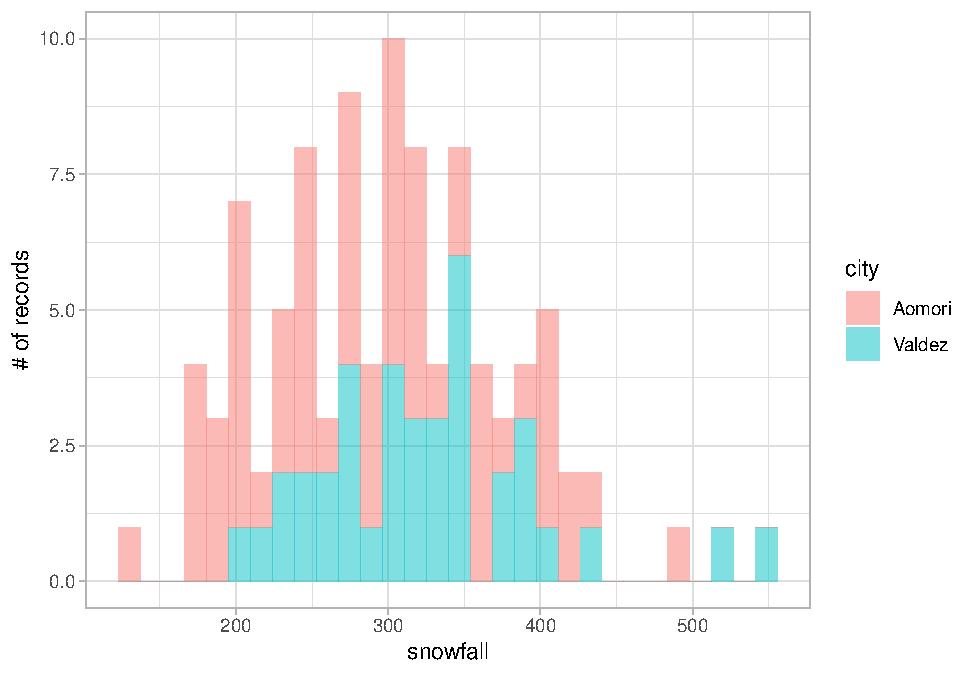
\includegraphics[width=0.33\linewidth]{fe_stat566_bak_files/figure-latex/unnamed-chunk-4-1}
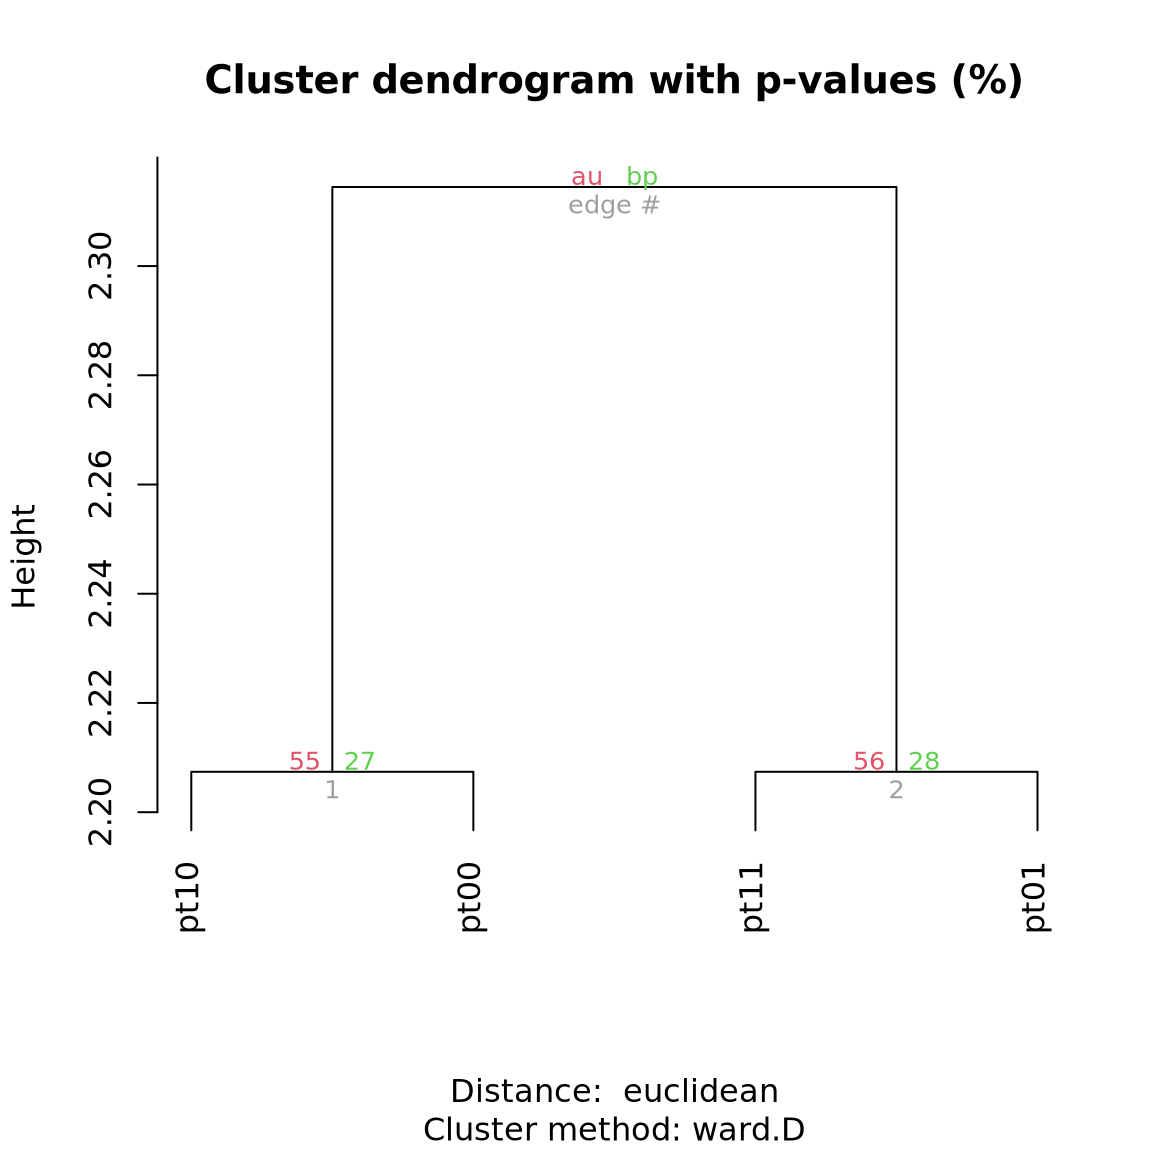
\includegraphics[width=0.33\linewidth]{fe_stat566_bak_files/figure-latex/unnamed-chunk-4-2}
\includegraphics[width=0.33\linewidth]{fe_stat566_bak_files/figure-latex/unnamed-chunk-4-3}

The above plots show that: The average purity analysed in Lab 1 is lower
than that from Lab 2. There is not much difference in the average purity
among technicians. The average purity of a chemical compound synthesized
from source 2 and 3 are higher than that from source 1. There is not
much difference in the average purity between sources 2 and 3.

\begin{table}[H]
\centering\begingroup\fontsize{8}{10}\selectfont

\begin{tabular}{lrrrrr>{\columncolor[HTML]{EAFAF1}}rrrr}
\toprule
Lab & min & Q1 & median & Q3 & max & mean & sd & n & missing\\
\midrule
1 & 8 & 13 & 17 & 21.0 & 30 & 17.00000 & 5.824352 & 27 & 0\\
2 & 10 & 15 & 20 & 23.5 & 29 & 19.25926 & 5.633639 & 27 & 0\\
\bottomrule
\end{tabular}
\endgroup{}
\end{table}

\begin{table}[H]
\centering\begingroup\fontsize{8}{10}\selectfont

\begin{tabular}{lrrrrr>{\columncolor[HTML]{EAFAF1}}rrrr}
\toprule
Technician & min & Q1 & median & Q3 & max & mean & sd & n & missing\\
\midrule
1 & 8 & 13.25 & 17 & 21.75 & 26 & 17.33333 & 5.718906 & 18 & 0\\
2 & 8 & 13.00 & 18 & 21.75 & 29 & 17.88889 & 6.057459 & 18 & 0\\
3 & 10 & 16.00 & 18 & 21.75 & 30 & 19.16667 & 5.762454 & 18 & 0\\
\bottomrule
\end{tabular}
\endgroup{}
\end{table}

\begin{table}[H]
\centering\begingroup\fontsize{8}{10}\selectfont

\begin{tabular}{lrrrrr>{\columncolor[HTML]{EAFAF1}}rrrr}
\toprule
Source & min & Q1 & median & Q3 & max & mean & sd & n & missing\\
\midrule
1 & 8 & 10.25 & 13.0 & 15.00 & 17 & 12.72222 & 2.803476 & 18 & 0\\
2 & 8 & 20.00 & 21.5 & 24.75 & 30 & 21.38889 & 5.326282 & 18 & 0\\
3 & 12 & 18.00 & 20.0 & 22.75 & 29 & 20.27778 & 4.599304 & 18 & 0\\
\bottomrule
\end{tabular}
\endgroup{}
\end{table}

There is not much difference in the average purity of sources 3 between
lab 1 and 2.

Not all the lines are parallel in the interaction plot. Therefore, in
the model, there is the interaction effect of source level and
technicians nested in the lab. The Tables show the same thing with the
numerical summaries for each factor level and their combinations.

\begin{table}[H]
\centering\begingroup\fontsize{8}{10}\selectfont

\begin{tabular}{lrrrrr>{\columncolor[HTML]{EAFAF1}}rrrr}
\toprule
Lab.Source & min & Q1 & median & Q3 & max & mean & sd & n & missing\\
\midrule
1.1 & 8 & 10 & 11 & 14 & 15 & 11.55556 & 2.505549 & 9 & 0\\
2.1 & 10 & 11 & 15 & 16 & 17 & 13.88889 & 2.713137 & 9 & 0\\
1.2 & 8 & 16 & 20 & 22 & 30 & 19.11111 & 6.392270 & 9 & 0\\
2.2 & 20 & 21 & 24 & 26 & 28 & 23.66667 & 2.783882 & 9 & 0\\
1.3 & 16 & 18 & 20 & 22 & 26 & 20.33333 & 3.500000 & 9 & 0\\
\addlinespace
2.3 & 12 & 18 & 20 & 23 & 29 & 20.22222 & 5.717906 & 9 & 0\\
\bottomrule
\end{tabular}
\endgroup{}
\end{table}

\begin{table}[H]
\centering\begingroup\fontsize{8}{10}\selectfont

\begin{tabular}{lrrrrr>{\columncolor[HTML]{EAFAF1}}rrrr}
\toprule
Technician.Source & min & Q1 & median & Q3 & max & mean & sd & n & missing\\
\midrule
1.1 & 9 & 10.75 & 14.0 & 15.00 & 17 & 13.16667 & 3.125167 & 6 & 0\\
2.1 & 8 & 10.25 & 11.0 & 12.50 & 15 & 11.33333 & 2.422120 & 6 & 0\\
3.1 & 10 & 11.75 & 14.0 & 15.50 & 17 & 13.66667 & 2.732520 & 6 & 0\\
1.2 & 8 & 20.00 & 20.5 & 23.25 & 26 & 19.83333 & 6.274286 & 6 & 0\\
2.2 & 13 & 21.25 & 23.0 & 24.75 & 26 & 21.83333 & 4.708149 & 6 & 0\\
\addlinespace
3.2 & 16 & 18.75 & 21.5 & 26.50 & 30 & 22.50000 & 5.504544 & 6 & 0\\
1.3 & 12 & 14.75 & 19.5 & 22.75 & 26 & 19.00000 & 5.513619 & 6 & 0\\
2.3 & 18 & 18.00 & 19.0 & 20.00 & 29 & 20.50000 & 4.277850 & 6 & 0\\
3.3 & 16 & 18.50 & 20.5 & 24.00 & 28 & 21.33333 & 4.457204 & 6 & 0\\
\bottomrule
\end{tabular}
\endgroup{}
\end{table}

This is a neseted and crossed design. Three fixed sources apply on all
random selected technicians nested in fixed labs.

\[y_{ijkl}=\mu+\tau_i+\beta_{j(i)}+\gamma_{k}+(\tau\gamma)_{ik}+(\beta\gamma)_{j(i)k}+\varepsilon_{(ijk)l}\]

for \(i=1,2\); \(j=1,2,3\); \(k=1,2,3\); \(l=1,2,3\);

\(\mu\) is the overall true mean response;

\(\tau_i\) is the fixed main effect of \(i^{th}\) level of labs;

\(\beta_{j(i)}\) is the random effect of \(j^{th}\) level of technicians
nested in \(i^{th}\) level of labs;

\(\gamma_{k}\) is the main fixed effect of \(k^{th}\) level of sources;

\((\tau\gamma)_{ik}\) is the interaction effect of \(i^{th}\) level of
labs and \(k^{th}\) level of sources;

\((\beta\gamma)_{j(i)k}\) is the interaction random effect of \(k^{th}\)
level of sources and \(j^{th}\) level of technicians nested in
\(i^{th}\) level of labs.

\(y_{ijkl}\) is response value for the \(l^{th}\) replication for
\(j^{th}\) level of technicians nested in \(i^{th}\) level of labs when
\(k^{th}\) level of sources is applied;

\(\varepsilon_{(ijk)l}\) is random error for the \(l^{th}\) replication
for \(j^{th}\) level of technicians nested in \(i^{th}\) level of labs
when \(k^{th}\) level of sources is applied.

Assumptions: Usually, the technicians in a lab are skillful. From the
above plots, the technicians' performances are stable. The covariance
between two observations from the same level of the random factor can be
either positive or negative. Thus we assume this is an
\textbf{restricted model}. \(\varepsilon_{(ijk)l}\), \(\beta_{j(i)}\),
and \((\beta\gamma)_{j(i)k}\) are independent.

\begin{longtable}[]{@{}llll@{}}
\toprule
\begin{minipage}[b]{0.19\columnwidth}\raggedright
\(\varepsilon_{(ijk)l}\sim iid N(0,\sigma^2)\)\strut
\end{minipage} & \begin{minipage}[b]{0.19\columnwidth}\raggedright
\(\sum_{i=1}^2\tau_{i}=0\)\strut
\end{minipage} & \begin{minipage}[b]{0.19\columnwidth}\raggedright
\(\sum_{k=1}^3\gamma_{k}=0\)\strut
\end{minipage} & \begin{minipage}[b]{0.32\columnwidth}\raggedright
\(\beta_{j(i)}\sim iid N(0,\sigma_{\beta}^2)\)\strut
\end{minipage}\tabularnewline
\midrule
\endhead
\begin{minipage}[t]{0.19\columnwidth}\raggedright
\(\sum_{i=1}^2(\tau\gamma)_{ik}=0\)\strut
\end{minipage} & \begin{minipage}[t]{0.19\columnwidth}\raggedright
\(\sum_{k=1}^3(\tau\gamma)_{ik}=0\)\strut
\end{minipage} & \begin{minipage}[t]{0.19\columnwidth}\raggedright
\(\sum_{i=1}^2(\beta\gamma)_{j(i)k}=0\)\strut
\end{minipage} & \begin{minipage}[t]{0.32\columnwidth}\raggedright
\((\beta\gamma)_{j(i)k}\sim iid N(0,\frac{2-1}{2}\sigma_{\beta\gamma}^2)\)\strut
\end{minipage}\tabularnewline
\bottomrule
\end{longtable}

\begin{longtable}[]{@{}cccccc@{}}
\caption{Analysis of Variance Table}\tabularnewline
\toprule
\begin{minipage}[b]{0.35\columnwidth}\centering
~\strut
\end{minipage} & \begin{minipage}[b]{0.05\columnwidth}\centering
Df\strut
\end{minipage} & \begin{minipage}[b]{0.09\columnwidth}\centering
Sum Sq\strut
\end{minipage} & \begin{minipage}[b]{0.10\columnwidth}\centering
Mean Sq\strut
\end{minipage} & \begin{minipage}[b]{0.10\columnwidth}\centering
F value\strut
\end{minipage} & \begin{minipage}[b]{0.12\columnwidth}\centering
Pr(\textgreater{}F)\strut
\end{minipage}\tabularnewline
\midrule
\endfirsthead
\toprule
\begin{minipage}[b]{0.35\columnwidth}\centering
~\strut
\end{minipage} & \begin{minipage}[b]{0.05\columnwidth}\centering
Df\strut
\end{minipage} & \begin{minipage}[b]{0.09\columnwidth}\centering
Sum Sq\strut
\end{minipage} & \begin{minipage}[b]{0.10\columnwidth}\centering
Mean Sq\strut
\end{minipage} & \begin{minipage}[b]{0.10\columnwidth}\centering
F value\strut
\end{minipage} & \begin{minipage}[b]{0.12\columnwidth}\centering
Pr(\textgreater{}F)\strut
\end{minipage}\tabularnewline
\midrule
\endhead
\begin{minipage}[t]{0.35\columnwidth}\centering
\textbf{Lab\_f}\strut
\end{minipage} & \begin{minipage}[t]{0.05\columnwidth}\centering
1\strut
\end{minipage} & \begin{minipage}[t]{0.09\columnwidth}\centering
68.91\strut
\end{minipage} & \begin{minipage}[t]{0.10\columnwidth}\centering
68.91\strut
\end{minipage} & \begin{minipage}[t]{0.10\columnwidth}\centering
6.955\strut
\end{minipage} & \begin{minipage}[t]{0.12\columnwidth}\centering
0.05775\strut
\end{minipage}\tabularnewline
\begin{minipage}[t]{0.35\columnwidth}\centering
\textbf{Source\_f}\strut
\end{minipage} & \begin{minipage}[t]{0.05\columnwidth}\centering
2\strut
\end{minipage} & \begin{minipage}[t]{0.09\columnwidth}\centering
800.6\strut
\end{minipage} & \begin{minipage}[t]{0.10\columnwidth}\centering
400.3\strut
\end{minipage} & \begin{minipage}[t]{0.10\columnwidth}\centering
30.62\strut
\end{minipage} & \begin{minipage}[t]{0.12\columnwidth}\centering
0.0001783\strut
\end{minipage}\tabularnewline
\begin{minipage}[t]{0.35\columnwidth}\centering
\textbf{Lab\_f:Source\_f}\strut
\end{minipage} & \begin{minipage}[t]{0.05\columnwidth}\centering
2\strut
\end{minipage} & \begin{minipage}[t]{0.09\columnwidth}\centering
49.04\strut
\end{minipage} & \begin{minipage}[t]{0.10\columnwidth}\centering
24.52\strut
\end{minipage} & \begin{minipage}[t]{0.10\columnwidth}\centering
1.875\strut
\end{minipage} & \begin{minipage}[t]{0.12\columnwidth}\centering
0.2148\strut
\end{minipage}\tabularnewline
\begin{minipage}[t]{0.35\columnwidth}\centering
\textbf{Lab\_f:Technician\_r}\strut
\end{minipage} & \begin{minipage}[t]{0.05\columnwidth}\centering
4\strut
\end{minipage} & \begin{minipage}[t]{0.09\columnwidth}\centering
39.63\strut
\end{minipage} & \begin{minipage}[t]{0.10\columnwidth}\centering
9.907\strut
\end{minipage} & \begin{minipage}[t]{0.10\columnwidth}\centering
0.5\strut
\end{minipage} & \begin{minipage}[t]{0.12\columnwidth}\centering
0.7358\strut
\end{minipage}\tabularnewline
\begin{minipage}[t]{0.35\columnwidth}\centering
\textbf{Lab\_f:Source\_f:Technician\_r}\strut
\end{minipage} & \begin{minipage}[t]{0.05\columnwidth}\centering
8\strut
\end{minipage} & \begin{minipage}[t]{0.09\columnwidth}\centering
104.6\strut
\end{minipage} & \begin{minipage}[t]{0.10\columnwidth}\centering
13.07\strut
\end{minipage} & \begin{minipage}[t]{0.10\columnwidth}\centering
0.6598\strut
\end{minipage} & \begin{minipage}[t]{0.12\columnwidth}\centering
0.7226\strut
\end{minipage}\tabularnewline
\begin{minipage}[t]{0.35\columnwidth}\centering
\textbf{Residual}\strut
\end{minipage} & \begin{minipage}[t]{0.05\columnwidth}\centering
36\strut
\end{minipage} & \begin{minipage}[t]{0.09\columnwidth}\centering
713.3\strut
\end{minipage} & \begin{minipage}[t]{0.10\columnwidth}\centering
19.81\strut
\end{minipage} & \begin{minipage}[t]{0.10\columnwidth}\centering
NA\strut
\end{minipage} & \begin{minipage}[t]{0.12\columnwidth}\centering
NA\strut
\end{minipage}\tabularnewline
\bottomrule
\end{longtable}

The ANOVA table shows that only sources have significant effects on the
average purity of a chemical compound synthesized at 0.05 significance
level (p-value=0.0001783).

\begin{longtable}[]{@{}lllll@{}}
\toprule
\begin{minipage}[b]{0.25\columnwidth}\raggedright
Groups Name\strut
\end{minipage} & \begin{minipage}[b]{0.13\columnwidth}\raggedright
\strut
\end{minipage} & \begin{minipage}[b]{0.09\columnwidth}\raggedright
Variance\strut
\end{minipage} & \begin{minipage}[b]{0.09\columnwidth}\raggedright
Std.Dev.\strut
\end{minipage} & \begin{minipage}[b]{0.28\columnwidth}\raggedright
\strut
\end{minipage}\tabularnewline
\midrule
\endhead
\begin{minipage}[t]{0.25\columnwidth}\raggedright
Source:Lab:Technician\strut
\end{minipage} & \begin{minipage}[t]{0.13\columnwidth}\raggedright
(Intercept)\strut
\end{minipage} & \begin{minipage}[t]{0.09\columnwidth}\raggedright
0.00\strut
\end{minipage} & \begin{minipage}[t]{0.09\columnwidth}\raggedright
0.000\strut
\end{minipage} & \begin{minipage}[t]{0.28\columnwidth}\raggedright
\(\sigma^2_{\beta\gamma}=0\)\strut
\end{minipage}\tabularnewline
\begin{minipage}[t]{0.25\columnwidth}\raggedright
Lab:Technician\strut
\end{minipage} & \begin{minipage}[t]{0.13\columnwidth}\raggedright
(Intercept)\strut
\end{minipage} & \begin{minipage}[t]{0.09\columnwidth}\raggedright
0.00\strut
\end{minipage} & \begin{minipage}[t]{0.09\columnwidth}\raggedright
0.000\strut
\end{minipage} & \begin{minipage}[t]{0.28\columnwidth}\raggedright
\(\sigma^2_{\beta}=0\)\strut
\end{minipage}\tabularnewline
\begin{minipage}[t]{0.25\columnwidth}\raggedright
Residual\strut
\end{minipage} & \begin{minipage}[t]{0.13\columnwidth}\raggedright
\strut
\end{minipage} & \begin{minipage}[t]{0.09\columnwidth}\raggedright
17.87\strut
\end{minipage} & \begin{minipage}[t]{0.09\columnwidth}\raggedright
4.227\strut
\end{minipage} & \begin{minipage}[t]{0.28\columnwidth}\raggedright
\(\sigma^2=17.87\)\strut
\end{minipage}\tabularnewline
\bottomrule
\end{longtable}

\begin{longtable}[]{@{}clll@{}}
\toprule
\begin{minipage}[b]{0.21\columnwidth}\centering
~\strut
\end{minipage} & \begin{minipage}[b]{0.10\columnwidth}\raggedright
2.5 \%\strut
\end{minipage} & \begin{minipage}[b]{0.09\columnwidth}\raggedright
97.5 \%\strut
\end{minipage} & \begin{minipage}[b]{0.48\columnwidth}\raggedright
\strut
\end{minipage}\tabularnewline
\midrule
\endhead
\begin{minipage}[t]{0.21\columnwidth}\centering
\textbf{.sig01}\strut
\end{minipage} & \begin{minipage}[t]{0.10\columnwidth}\raggedright
0\strut
\end{minipage} & \begin{minipage}[t]{0.09\columnwidth}\raggedright
1.539\strut
\end{minipage} & \begin{minipage}[t]{0.48\columnwidth}\raggedright
\(CI_{\sigma^2_{\beta\gamma}}:(0,1.539^2)\)\strut
\end{minipage}\tabularnewline
\begin{minipage}[t]{0.21\columnwidth}\centering
\textbf{.sig02}\strut
\end{minipage} & \begin{minipage}[t]{0.10\columnwidth}\raggedright
0\strut
\end{minipage} & \begin{minipage}[t]{0.09\columnwidth}\raggedright
1.603\strut
\end{minipage} & \begin{minipage}[t]{0.48\columnwidth}\raggedright
\(CI_{\sigma^2_{\beta}}:(0,1.603^2)\)\strut
\end{minipage}\tabularnewline
\begin{minipage}[t]{0.21\columnwidth}\centering
\textbf{.sigma}\strut
\end{minipage} & \begin{minipage}[t]{0.10\columnwidth}\raggedright
3.337\strut
\end{minipage} & \begin{minipage}[t]{0.09\columnwidth}\raggedright
4.873\strut
\end{minipage} & \begin{minipage}[t]{0.48\columnwidth}\raggedright
\(CI_{\sigma^2}:(3.337^2,4.873^2)\)\strut
\end{minipage}\tabularnewline
\bottomrule
\end{longtable}

The results of variance components and condidence intervals show that
none of the effects related with technician has significant variance on
average value of purity at 0.05 significance level. The variance of
interaction effect between sources and technicians nested in labs is
zero with confidence intervals (\(0,1.539^2\)) at 0.05 significance
level. The variance of technicians nested in labs is zero with
confidence intervals (\(0,1.603^2\)) at 0.05 significance level.

\textbf{Conclusion:} As the main effects of sources shown in the above
tables, the average purity is different with sources. The average purity
from source 1 is lowest (12.72222). The the average purity from source 2
and 3 are 21.38889 and 20.27778 respectively. The selections of labs and
technicians don't change this result.

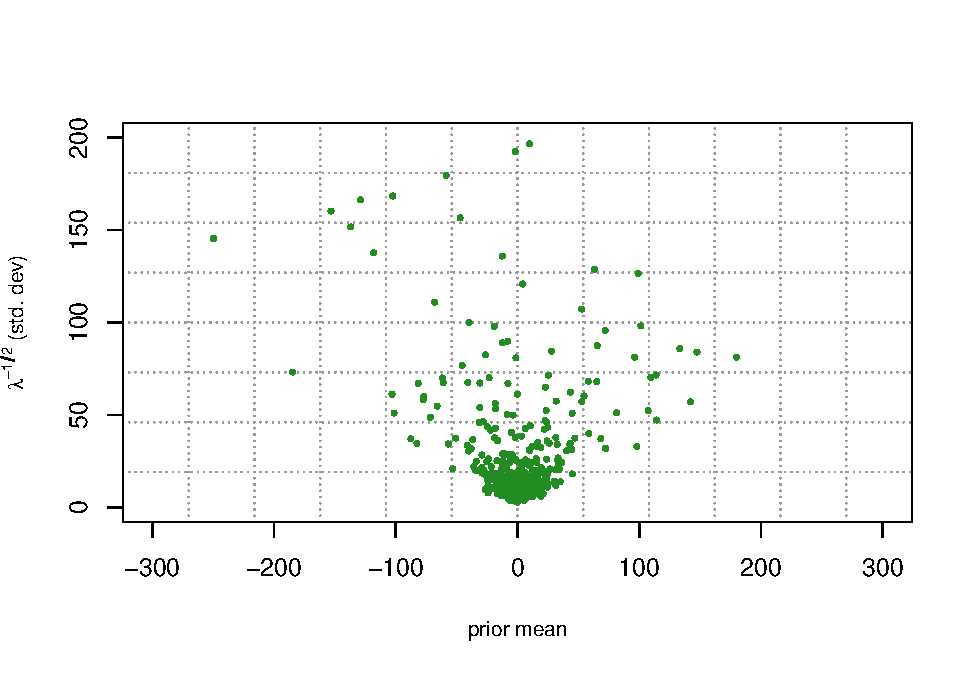
\includegraphics[width=0.25\linewidth]{fe_stat566_bak_files/figure-latex/unnamed-chunk-12-1}
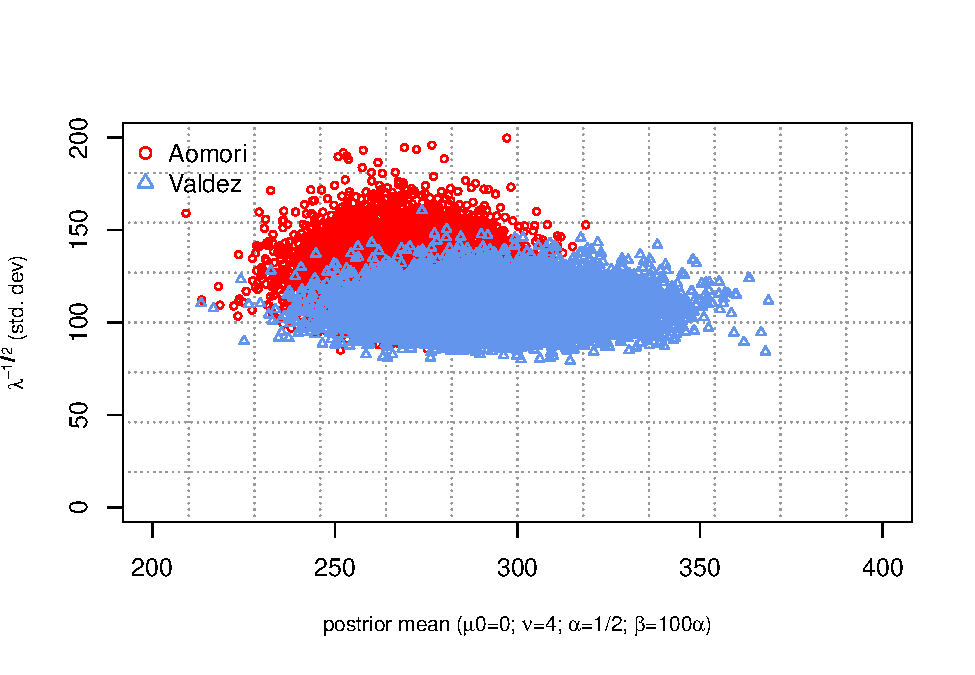
\includegraphics[width=0.25\linewidth]{fe_stat566_bak_files/figure-latex/unnamed-chunk-12-2}
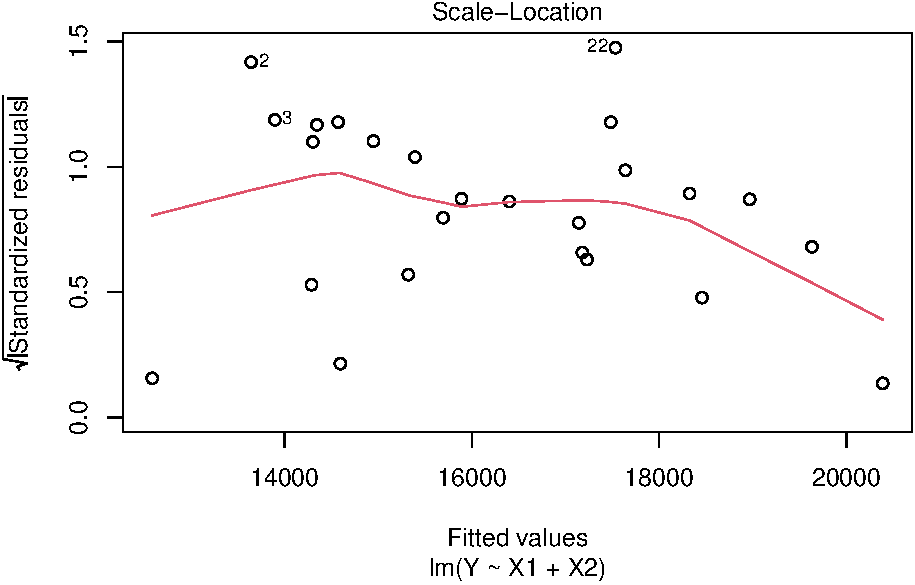
\includegraphics[width=0.25\linewidth]{fe_stat566_bak_files/figure-latex/unnamed-chunk-12-3}
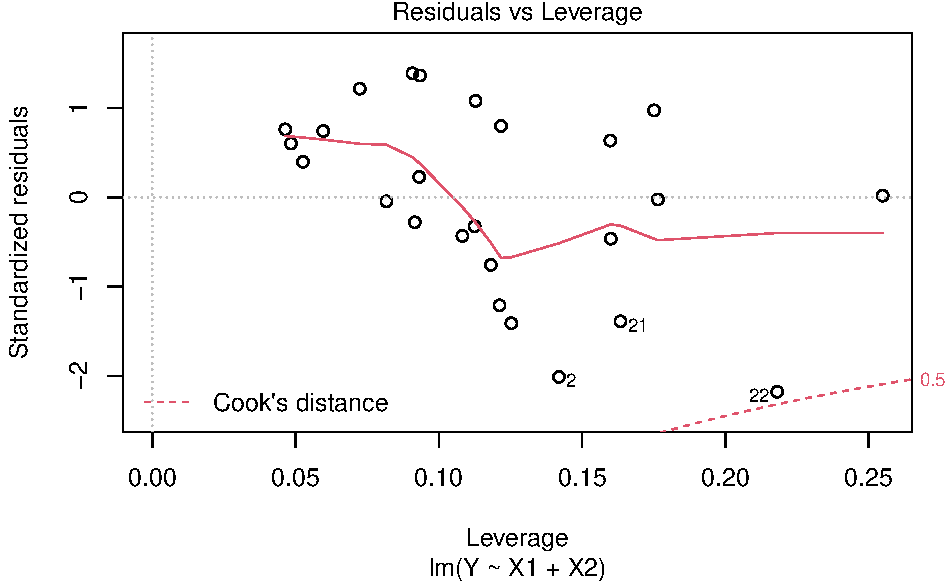
\includegraphics[width=0.25\linewidth]{fe_stat566_bak_files/figure-latex/unnamed-chunk-12-4}

In the plots of residuals versus predicted value of purity, there is no
significant pattern on this plot besides that more values occur when the
predicted value is higher. Therefore, the fitted model is good enough to
describe the relationship between the mean value of purity and the labs,
technician, and sources.

The residuals in this plot are almost symmetrically distributed about
zero and hence zero mean assumption is not violated. Further, the
vertical deviation of the residuals from zero is about same for each
predicted value and hence the constant variance assumption is not
violated.

The points are along the straight line in the normal qq plot shown at
bottom left and the histogram of residuals shown at the top right is
about normal. These plots show no violation of normal distribution
assumption of residuals.

\textcolor[rgb]{0.7,0.7,0.7}{Report your code and/or output at the end of the analysis.}

\begin{Shaded}
\begin{Highlighting}[]
\KeywordTok{favstats}\NormalTok{(Purity }\OperatorTok{~}\StringTok{ }\NormalTok{Source, }\DataTypeTok{data =}\NormalTok{ fe_table_chem)}
\KeywordTok{favstats}\NormalTok{(Purity }\OperatorTok{~}\StringTok{ }\NormalTok{Lab, }\DataTypeTok{data =}\NormalTok{ fe_table_chem)}
\KeywordTok{favstats}\NormalTok{(Purity }\OperatorTok{~}\StringTok{ }\NormalTok{Lab }\OperatorTok{+}\StringTok{ }\NormalTok{Source, }\DataTypeTok{data =}\NormalTok{ fe_table_chem)}
\KeywordTok{favstats}\NormalTok{(Purity }\OperatorTok{~}\StringTok{ }\NormalTok{Technician, }\DataTypeTok{data =}\NormalTok{ fe_table_chem)}
\KeywordTok{favstats}\NormalTok{(Purity }\OperatorTok{~}\StringTok{ }\NormalTok{Technician }\OperatorTok{+}\StringTok{ }\NormalTok{Source, }\DataTypeTok{data =}\NormalTok{ fe_table_chem)}
\NormalTok{fe_table_chem}\OperatorTok{$}\NormalTok{Lab_f <-}\StringTok{ }\KeywordTok{as.fixed}\NormalTok{(fe_table_chem}\OperatorTok{$}\NormalTok{Lab)}
\NormalTok{fe_table_chem}\OperatorTok{$}\NormalTok{Technician_r <-}\StringTok{ }\KeywordTok{as.random}\NormalTok{(fe_table_chem}\OperatorTok{$}\NormalTok{Technician)}
\NormalTok{fe_table_chem}\OperatorTok{$}\NormalTok{Source_f <-}\StringTok{ }\KeywordTok{as.fixed}\NormalTok{(fe_table_chem}\OperatorTok{$}\NormalTok{Source)}
\NormalTok{fe_model_chem1 <-}\StringTok{ }\KeywordTok{aov}\NormalTok{(}\DataTypeTok{formula =}\NormalTok{ Purity }\OperatorTok{~}\StringTok{ }\NormalTok{Lab_f }\OperatorTok{*}\StringTok{ }\NormalTok{Source_f }\OperatorTok{+}\StringTok{ }\NormalTok{Technician_r }\OperatorTok\StringTok{ }
\StringTok{    }\NormalTok{Lab_f }\OperatorTok{+}\StringTok{ }\NormalTok{Source_f }\OperatorTok{*}\StringTok{ }\NormalTok{Technician_r }\OperatorTok\StringTok{ }\NormalTok{Lab_f, }\DataTypeTok{data =}\NormalTok{ fe_table_chem)}
\KeywordTok{gad}\NormalTok{(fe_model_chem1)}

\NormalTok{fe_model_chem2 <-}\StringTok{ }\KeywordTok{lmer}\NormalTok{(}\DataTypeTok{formula =}\NormalTok{ Purity }\OperatorTok{~}\StringTok{ }\NormalTok{Lab }\OperatorTok{*}\StringTok{ }\NormalTok{Source }\OperatorTok{+}\StringTok{ }\NormalTok{(}\DecValTok{1} \OperatorTok{|}\StringTok{ }\NormalTok{Lab}\OperatorTok{:}\NormalTok{Technician) }\OperatorTok{+}\StringTok{ }
\StringTok{    }\NormalTok{(}\DecValTok{1} \OperatorTok{|}\StringTok{ }\NormalTok{Source}\OperatorTok{:}\NormalTok{Lab}\OperatorTok{:}\NormalTok{Technician), }\DataTypeTok{data =}\NormalTok{ fe_table_chem, }\DataTypeTok{REML =} \OtherTok{TRUE}\NormalTok{)}
\KeywordTok{summary}\NormalTok{(fe_model_chem2)}
\KeywordTok{confint}\NormalTok{(fe_model_chem2)}

\NormalTok{fe_residual_chem <-}\StringTok{ }\KeywordTok{rstudent}\NormalTok{(fe_model_chem2)}
\KeywordTok{plot}\NormalTok{(fe_residual_chem)}
\KeywordTok{plot}\NormalTok{(fe_model_chem2)}
\KeywordTok{qqnorm}\NormalTok{(fe_residual_chem)}
\KeywordTok{qqline}\NormalTok{(fe_residual_chem)}
\KeywordTok{hist}\NormalTok{(fe_residual_chem)}
\end{Highlighting}
\end{Shaded}

\hypertarget{question-4}{%
\subsubsection{Question 4}\label{question-4}}

\textcolor[rgb]{0.7,0.7,0.7}{A baker wanted to determine the effect that the amount of fat in a recipe of cookie dough would have on the texture of the cookie. The baker also wanted to determine whether the temperature (°F) at which the cookies were baked would have an influence on the texture of the surface. The texture of the cookie is measured by determining the amount of force (g) required to penetrate the cookie surface.}
\textcolor[rgb]{0.7,0.7,0.7}{On a given day, the baker made a batch of cookie dough for each of the 4 recipes and baked one cookie from each batch in the oven at one time. The baker continued this process each of 4 days so that a single cookie is baked at 3 different temperatures in one day.The data are given in Cookie Excel file.}
\textcolor[rgb]{0.7,0.7,0.7}{Analyze the data and answer the baker's questions. If you have to decide between unrestricted and restricted models, then make a decision and provide reasons.}

\begin{verbatim}
## Classes 'tbl_df', 'tbl' and 'data.frame':    48 obs. of  4 variables:
##  $ day  : Factor w/ 4 levels "1","2","3","4": 1 1 1 1 1 1 1 1 1 1 ...
##  $ temp : Factor w/ 3 levels "350","375","400": 1 1 1 1 2 2 2 2 3 3 ...
##  $ fat  : Factor w/ 4 levels "2","4","6","8": 1 2 3 4 1 2 3 4 1 2 ...
##  $ force: num  7.4 7.1 7.2 6.7 11.2 11.1 10.6 10.8 11.8 11.2 ...
\end{verbatim}

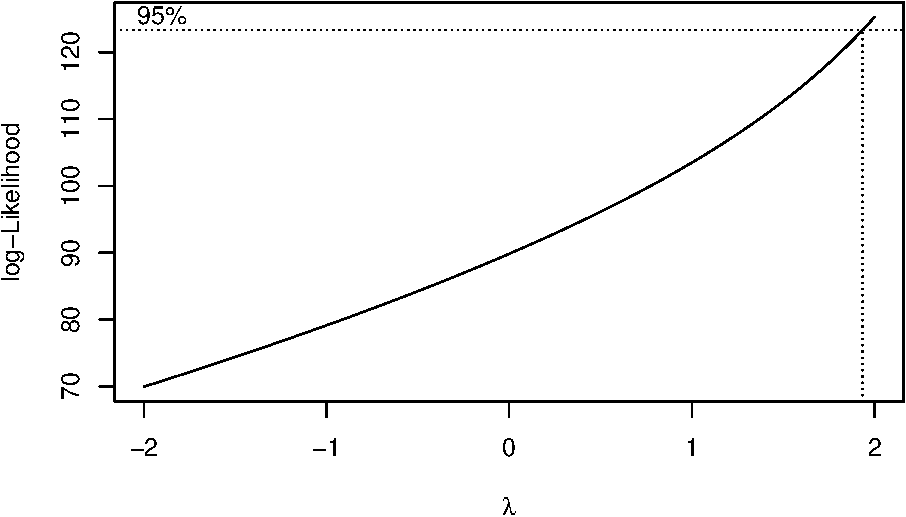
\includegraphics[width=0.3\linewidth]{fe_stat566_bak_files/figure-latex/unnamed-chunk-14-1}
\includegraphics[width=0.3\linewidth]{fe_stat566_bak_files/figure-latex/unnamed-chunk-14-2}
\includegraphics[width=0.3\linewidth]{fe_stat566_bak_files/figure-latex/unnamed-chunk-14-3}

The above plots show that: There is not much difference in the average
force of the cookie from different days or form different fat. The
tables show the same thing with the numerical summaries for each factor
level and their combinations. The average force of the cookie are higher
when the temperature is higher.

\begin{table}[H]
\centering\begingroup\fontsize{8}{10}\selectfont

\begin{tabular}{lrrrrr>{\columncolor[HTML]{EAFAF1}}rrrr}
\toprule
day & min & Q1 & median & Q3 & max & mean & sd & n & missing\\
\midrule
1 & 6.7 & 7.35 & 10.95 & 11.225 & 11.8 & 9.816667 & 2.033284 & 12 & 0\\
2 & 7.2 & 8.55 & 10.15 & 12.750 & 14.0 & 10.475000 & 2.384467 & 12 & 0\\
3 & 6.1 & 6.85 & 8.00 & 12.025 & 12.2 & 8.825000 & 2.526271 & 12 & 0\\
4 & 6.0 & 6.85 & 8.20 & 11.475 & 12.1 & 8.900000 & 2.290693 & 12 & 0\\
\bottomrule
\end{tabular}
\endgroup{}
\end{table}

\begin{table}[H]
\centering\begingroup\fontsize{8}{10}\selectfont

\begin{tabular}{lrrrrr>{\columncolor[HTML]{EAFAF1}}rrrr}
\toprule
fat & min & Q1 & median & Q3 & max & mean & sd & n & missing\\
\midrule
2 & 6.6 & 8.075 & 9.95 & 11.725 & 12.9 & 9.800000 & 2.200413 & 12 & 0\\
4 & 6.4 & 7.550 & 9.10 & 11.425 & 14.0 & 9.558333 & 2.520988 & 12 & 0\\
6 & 6.2 & 7.350 & 9.15 & 11.450 & 13.6 & 9.416667 & 2.480408 & 12 & 0\\
8 & 6.0 & 7.075 & 9.30 & 11.400 & 12.7 & 9.241667 & 2.439992 & 12 & 0\\
\bottomrule
\end{tabular}
\endgroup{}
\end{table}

\begin{table}[H]
\centering\begingroup\fontsize{8}{10}\selectfont

\begin{tabular}{lrrrrr>{\columncolor[HTML]{EAFAF1}}rrrr}
\toprule
temp & min & Q1 & median & Q3 & max & mean & sd & n & missing\\
\midrule
350 & 6.0 & 6.550 & 6.95 & 7.250 & 8.7 & 6.98125 & 0.7148135 & 16 & 0\\
375 & 7.4 & 8.250 & 9.55 & 10.650 & 11.2 & 9.38125 & 1.3422463 & 16 & 0\\
400 & 11.2 & 11.625 & 12.05 & 12.325 & 14.0 & 12.15000 & 0.7983316 & 16 & 0\\
\bottomrule
\end{tabular}
\endgroup{}
\end{table}

Not all the lines are parallel in the interaction plot. Therefore, in
the model, there is the interaction effect of day and temperature.

\begin{table}[H]
\centering\begingroup\fontsize{8}{10}\selectfont

\begin{tabular}{lrrrrr>{\columncolor[HTML]{EAFAF1}}rrrr}
\toprule
day.fat & min & Q1 & median & Q3 & max & mean & sd & n & missing\\
\midrule
1.2 & 7.4 & 9.30 & 11.2 & 11.50 & 11.8 & 10.133333 & 2.386071 & 3 & 0\\
2.2 & 8.7 & 9.75 & 10.8 & 11.85 & 12.9 & 10.800000 & 2.100000 & 3 & 0\\
3.2 & 7.0 & 7.65 & 8.3 & 10.20 & 12.1 & 9.133333 & 2.650157 & 3 & 0\\
4.2 & 6.6 & 7.85 & 9.1 & 10.40 & 11.7 & 9.133333 & 2.550163 & 3 & 0\\
1.4 & 7.1 & 9.10 & 11.1 & 11.15 & 11.2 & 9.800000 & 2.338803 & 3 & 0\\
\addlinespace
2.4 & 8.1 & 9.10 & 10.1 & 12.05 & 14.0 & 10.733333 & 3.000555 & 3 & 0\\
3.4 & 6.4 & 7.05 & 7.7 & 9.90 & 12.1 & 8.733333 & 2.987195 & 3 & 0\\
4.4 & 6.7 & 7.40 & 8.1 & 10.10 & 12.1 & 8.966667 & 2.802380 & 3 & 0\\
1.6 & 7.2 & 8.90 & 10.6 & 10.95 & 11.3 & 9.700000 & 2.193171 & 3 & 0\\
2.6 & 7.4 & 8.70 & 10.0 & 11.80 & 13.6 & 10.333333 & 3.113412 & 3 & 0\\
\addlinespace
3.6 & 6.2 & 6.80 & 7.4 & 9.80 & 12.2 & 8.600000 & 3.174902 & 3 & 0\\
4.6 & 6.9 & 7.60 & 8.3 & 10.10 & 11.9 & 9.033333 & 2.579406 & 3 & 0\\
1.8 & 6.7 & 8.75 & 10.8 & 11.10 & 11.4 & 9.633333 & 2.557994 & 3 & 0\\
2.8 & 7.2 & 8.70 & 10.2 & 11.45 & 12.7 & 10.033333 & 2.753785 & 3 & 0\\
3.8 & 6.1 & 7.25 & 8.4 & 10.20 & 12.0 & 8.833333 & 2.973774 & 3 & 0\\
\addlinespace
4.8 & 6.0 & 7.00 & 8.0 & 9.70 & 11.4 & 8.466667 & 2.730079 & 3 & 0\\
\bottomrule
\end{tabular}
\endgroup{}
\end{table}

\begin{table}[H]
\centering\begingroup\fontsize{8}{10}\selectfont

\begin{tabular}{lrrrrr>{\columncolor[HTML]{EAFAF1}}rrrr}
\toprule
temp.fat & min & Q1 & median & Q3 & max & mean & sd & n & missing\\
\midrule
350.2 & 6.6 & 6.900 & 7.20 & 7.725 & 8.7 & 7.425 & 0.9105859 & 4 & 0\\
375.2 & 8.3 & 8.900 & 9.95 & 10.900 & 11.2 & 9.850 & 1.3771952 & 4 & 0\\
400.2 & 11.7 & 11.775 & 11.95 & 12.300 & 12.9 & 12.125 & 0.5439056 & 4 & 0\\
350.4 & 6.4 & 6.625 & 6.90 & 7.350 & 8.1 & 7.075 & 0.7410578 & 4 & 0\\
375.4 & 7.7 & 8.000 & 9.10 & 10.350 & 11.1 & 9.250 & 1.6196707 & 4 & 0\\
\addlinespace
400.4 & 11.2 & 11.875 & 12.10 & 12.575 & 14.0 & 12.350 & 1.1789826 & 4 & 0\\
350.6 & 6.2 & 6.725 & 7.05 & 7.250 & 7.4 & 6.925 & 0.5251984 & 4 & 0\\
375.6 & 7.4 & 8.075 & 9.15 & 10.150 & 10.6 & 9.075 & 1.4818344 & 4 & 0\\
400.6 & 11.3 & 11.750 & 12.05 & 12.550 & 13.6 & 12.250 & 0.9746794 & 4 & 0\\
350.8 & 6.0 & 6.075 & 6.40 & 6.825 & 7.2 & 6.500 & 0.5597619 & 4 & 0\\
\addlinespace
375.8 & 8.0 & 8.300 & 9.30 & 10.350 & 10.8 & 9.350 & 1.3601471 & 4 & 0\\
400.8 & 11.4 & 11.400 & 11.70 & 12.175 & 12.7 & 11.875 & 0.6184658 & 4 & 0\\
\bottomrule
\end{tabular}
\endgroup{}
\end{table}

\begin{table}[H]
\centering\begingroup\fontsize{8}{10}\selectfont

\begin{tabular}{lrrrrr>{\columncolor[HTML]{EAFAF1}}rrrr}
\toprule
temp.day & min & Q1 & median & Q3 & max & mean & sd & n & missing\\
\midrule
350.1 & 6.7 & 7.000 & 7.15 & 7.250 & 7.4 & 7.100 & 0.2943920 & 4 & 0\\
375.1 & 10.6 & 10.750 & 10.95 & 11.125 & 11.2 & 10.925 & 0.2753785 & 4 & 0\\
400.1 & 11.2 & 11.275 & 11.35 & 11.500 & 11.8 & 11.425 & 0.2629956 & 4 & 0\\
350.2 & 7.2 & 7.350 & 7.75 & 8.250 & 8.7 & 7.850 & 0.6855655 & 4 & 0\\
375.2 & 10.0 & 10.075 & 10.15 & 10.350 & 10.8 & 10.275 & 0.3593976 & 4 & 0\\
\addlinespace
400.2 & 12.7 & 12.850 & 13.25 & 13.700 & 14.0 & 13.300 & 0.6055301 & 4 & 0\\
350.3 & 6.1 & 6.175 & 6.30 & 6.550 & 7.0 & 6.425 & 0.4031129 & 4 & 0\\
375.3 & 7.4 & 7.625 & 8.00 & 8.325 & 8.4 & 7.950 & 0.4795832 & 4 & 0\\
400.3 & 12.0 & 12.075 & 12.10 & 12.125 & 12.2 & 12.100 & 0.0816497 & 4 & 0\\
350.4 & 6.0 & 6.450 & 6.65 & 6.750 & 6.9 & 6.550 & 0.3872983 & 4 & 0\\
\addlinespace
375.4 & 8.0 & 8.075 & 8.20 & 8.500 & 9.1 & 8.375 & 0.4991660 & 4 & 0\\
400.4 & 11.4 & 11.625 & 11.80 & 11.950 & 12.1 & 11.775 & 0.2986079 & 4 & 0\\
\bottomrule
\end{tabular}
\endgroup{}
\end{table}

This is a simple Split-Plot design model (fat is whole-plot factor and
temperature is split-plot factor)

\[y_{ijk}=\mu+\tau_i+\beta_{j}+(\tau\beta)_{ij}+\gamma_{k}+(\tau\gamma)_{ik}+(\beta\gamma)_{jk}+(\tau\beta\gamma)_{ijk}+\varepsilon_{ijk}\]

for \(i=1,2,3,4\); \(j=1,2,3\); \(k=1,2,3,4\)

\(\mu\) is the overall true mean response;

\(\tau_i\) is the effect of \(i^{th}\) replication of days;

\(\beta_{j}\) is the main effect of \(j^{th}\) level of temperature
(effect of split-plot factor);

\((\tau\beta)_{ij}\) is the interaction effect of \(i^{th}\) replication
and \(j^{th}\) level of temperature;

\(\gamma_{k}\) is the main effect of \(k^{th}\) level of fat (effect of
whole-plot factor);

\((\tau\gamma)_{ik}\) is the interaction effect of \(i^{th}\) replicatin
and \(k^{th}\) level of fat(whole-plot error);

\((\beta\gamma)_{jk}\) is the interaction effect of \(j^{th}\) level of
temperature and \(k^{th}\) level of fat;

\((\tau\beta\gamma)_{ijk}\) is the interaction effect of \(i^{th}\)
replicatin, \(j^{th}\) level of temperature and \(k^{th}\) level of fat
(sub-plot error);

\(y_{ijk}\) is response value for the \(i^{th}\) replication when
\(j^{th}\) level of temperature and \(k^{th}\) level of fat are applied;

\(\varepsilon_{ijk}\) is random error for the \(i^{th}\) replication
when \(j^{th}\) level of temperature and \(k^{th}\) level of fat are
applied.

Assumptions: For an experienced baker, he/she will try to let the recipe
and temperature are accurate in each day. the covariance between two
observations from the same level of the random factor can be either
positive or negative. Thus, we assume this is a \textbf{restricted
model}.

\begin{longtable}[]{@{}lll@{}}
\toprule
\begin{minipage}[b]{0.23\columnwidth}\raggedright
\(\varepsilon_{ijk}\sim iid N(0,\sigma^2)\)\strut
\end{minipage} & \begin{minipage}[b]{0.23\columnwidth}\raggedright
\(\tau_i\sim iid N(0,\sigma_{\tau}^2)\)\strut
\end{minipage} & \begin{minipage}[b]{0.46\columnwidth}\raggedright
\strut
\end{minipage}\tabularnewline
\midrule
\endhead
\begin{minipage}[t]{0.23\columnwidth}\raggedright
\(\sum_{j=1}^3\beta_{j}=0\)\strut
\end{minipage} & \begin{minipage}[t]{0.23\columnwidth}\raggedright
\(\sum_{j=1}^3(\tau\beta)_{ij}=0\)\strut
\end{minipage} & \begin{minipage}[t]{0.46\columnwidth}\raggedright
\((\tau\beta)_{ij}\sim iid N(0,\frac{3-1}{3}\sigma_{\tau\beta}^2)\)\strut
\end{minipage}\tabularnewline
\begin{minipage}[t]{0.23\columnwidth}\raggedright
\(\sum_{k=1}^4\gamma_{k}=0\)\strut
\end{minipage} & \begin{minipage}[t]{0.23\columnwidth}\raggedright
\(\sum_{k=1}^4(\tau\gamma)_{ik}=0\)\strut
\end{minipage} & \begin{minipage}[t]{0.46\columnwidth}\raggedright
\((\tau\gamma)_{ik}\sim iid N(0,\frac{4-1}{4}\sigma_{\tau\gamma}^2)\)\strut
\end{minipage}\tabularnewline
\begin{minipage}[t]{0.23\columnwidth}\raggedright
\(\sum_{j=1}^3(\beta\gamma)_{jk}=0\)\strut
\end{minipage} & \begin{minipage}[t]{0.23\columnwidth}\raggedright
\(\sum_{k=1}^4(\beta\gamma)_{jk}=0\)\strut
\end{minipage} & \begin{minipage}[t]{0.46\columnwidth}\raggedright
\strut
\end{minipage}\tabularnewline
\begin{minipage}[t]{0.23\columnwidth}\raggedright
\(\sum_{j=1}^3(\tau\beta\gamma)_{ijk}=0\)\strut
\end{minipage} & \begin{minipage}[t]{0.23\columnwidth}\raggedright
\(\sum_{k=1}^4(\tau\beta\gamma)_{ijk}=0\)\strut
\end{minipage} & \begin{minipage}[t]{0.46\columnwidth}\raggedright
\((\tau\beta\gamma)_{ijk}\sim iid N(0,\frac{(3-1)(4-1)}{3\times4}\sigma_{\tau\beta\gamma}^2)\)\strut
\end{minipage}\tabularnewline
\bottomrule
\end{longtable}

\(\varepsilon_{ijk}\), \(\tau_{i}\), \((\tau\beta)_{ij}\),
\((\tau\gamma)_{ik}\), \((\beta\gamma)_{jk}\), and
\((\tau\beta\gamma)_{ijk}\) are independent.

Since this is a simple replicated factorial design, I use
\((\tau\beta\gamma)_{ijk}\) to compute SSE and df.

\begin{longtable}[]{@{}cccccc@{}}
\caption{Analysis of Variance Table}\tabularnewline
\toprule
\begin{minipage}[b]{0.22\columnwidth}\centering
~\strut
\end{minipage} & \begin{minipage}[b]{0.06\columnwidth}\centering
Df\strut
\end{minipage} & \begin{minipage}[b]{0.10\columnwidth}\centering
Sum Sq\strut
\end{minipage} & \begin{minipage}[b]{0.12\columnwidth}\centering
Mean Sq\strut
\end{minipage} & \begin{minipage}[b]{0.12\columnwidth}\centering
F value\strut
\end{minipage} & \begin{minipage}[b]{0.14\columnwidth}\centering
Pr(\textgreater{}F)\strut
\end{minipage}\tabularnewline
\midrule
\endfirsthead
\toprule
\begin{minipage}[b]{0.22\columnwidth}\centering
~\strut
\end{minipage} & \begin{minipage}[b]{0.06\columnwidth}\centering
Df\strut
\end{minipage} & \begin{minipage}[b]{0.10\columnwidth}\centering
Sum Sq\strut
\end{minipage} & \begin{minipage}[b]{0.12\columnwidth}\centering
Mean Sq\strut
\end{minipage} & \begin{minipage}[b]{0.12\columnwidth}\centering
F value\strut
\end{minipage} & \begin{minipage}[b]{0.14\columnwidth}\centering
Pr(\textgreater{}F)\strut
\end{minipage}\tabularnewline
\midrule
\endhead
\begin{minipage}[t]{0.22\columnwidth}\centering
\textbf{day\_r}\strut
\end{minipage} & \begin{minipage}[t]{0.06\columnwidth}\centering
3\strut
\end{minipage} & \begin{minipage}[t]{0.10\columnwidth}\centering
22.4\strut
\end{minipage} & \begin{minipage}[t]{0.12\columnwidth}\centering
7.466\strut
\end{minipage} & \begin{minipage}[t]{0.12\columnwidth}\centering
74.5\strut
\end{minipage} & \begin{minipage}[t]{0.14\columnwidth}\centering
2.415e-10\strut
\end{minipage}\tabularnewline
\begin{minipage}[t]{0.22\columnwidth}\centering
\textbf{fat\_f}\strut
\end{minipage} & \begin{minipage}[t]{0.06\columnwidth}\centering
3\strut
\end{minipage} & \begin{minipage}[t]{0.10\columnwidth}\centering
2.004\strut
\end{minipage} & \begin{minipage}[t]{0.12\columnwidth}\centering
0.6681\strut
\end{minipage} & \begin{minipage}[t]{0.12\columnwidth}\centering
7.012\strut
\end{minipage} & \begin{minipage}[t]{0.14\columnwidth}\centering
0.009915\strut
\end{minipage}\tabularnewline
\begin{minipage}[t]{0.22\columnwidth}\centering
\textbf{temp\_f}\strut
\end{minipage} & \begin{minipage}[t]{0.06\columnwidth}\centering
2\strut
\end{minipage} & \begin{minipage}[t]{0.10\columnwidth}\centering
214.1\strut
\end{minipage} & \begin{minipage}[t]{0.12\columnwidth}\centering
107\strut
\end{minipage} & \begin{minipage}[t]{0.12\columnwidth}\centering
41.18\strut
\end{minipage} & \begin{minipage}[t]{0.14\columnwidth}\centering
0.0003131\strut
\end{minipage}\tabularnewline
\begin{minipage}[t]{0.22\columnwidth}\centering
\textbf{day\_r:fat\_f}\strut
\end{minipage} & \begin{minipage}[t]{0.06\columnwidth}\centering
9\strut
\end{minipage} & \begin{minipage}[t]{0.10\columnwidth}\centering
0.8575\strut
\end{minipage} & \begin{minipage}[t]{0.12\columnwidth}\centering
0.09528\strut
\end{minipage} & \begin{minipage}[t]{0.12\columnwidth}\centering
0.9508\strut
\end{minipage} & \begin{minipage}[t]{0.14\columnwidth}\centering
0.5082\strut
\end{minipage}\tabularnewline
\begin{minipage}[t]{0.22\columnwidth}\centering
\textbf{day\_r:temp\_f}\strut
\end{minipage} & \begin{minipage}[t]{0.06\columnwidth}\centering
6\strut
\end{minipage} & \begin{minipage}[t]{0.10\columnwidth}\centering
15.6\strut
\end{minipage} & \begin{minipage}[t]{0.12\columnwidth}\centering
2.599\strut
\end{minipage} & \begin{minipage}[t]{0.12\columnwidth}\centering
25.94\strut
\end{minipage} & \begin{minipage}[t]{0.14\columnwidth}\centering
6.251e-08\strut
\end{minipage}\tabularnewline
\begin{minipage}[t]{0.22\columnwidth}\centering
\textbf{fat\_f:temp\_f}\strut
\end{minipage} & \begin{minipage}[t]{0.06\columnwidth}\centering
6\strut
\end{minipage} & \begin{minipage}[t]{0.10\columnwidth}\centering
1.59\strut
\end{minipage} & \begin{minipage}[t]{0.12\columnwidth}\centering
0.2649\strut
\end{minipage} & \begin{minipage}[t]{0.12\columnwidth}\centering
2.644\strut
\end{minipage} & \begin{minipage}[t]{0.14\columnwidth}\centering
0.05113\strut
\end{minipage}\tabularnewline
\begin{minipage}[t]{0.22\columnwidth}\centering
\textbf{Residual}\strut
\end{minipage} & \begin{minipage}[t]{0.06\columnwidth}\centering
18\strut
\end{minipage} & \begin{minipage}[t]{0.10\columnwidth}\centering
1.804\strut
\end{minipage} & \begin{minipage}[t]{0.12\columnwidth}\centering
0.1002\strut
\end{minipage} & \begin{minipage}[t]{0.12\columnwidth}\centering
NA\strut
\end{minipage} & \begin{minipage}[t]{0.14\columnwidth}\centering
NA\strut
\end{minipage}\tabularnewline
\bottomrule
\end{longtable}

The results show the interaction effect of day and fat is not
significant at 0.05 significance level (P-value=0.5082).

The interaction effect of day and temperature is significant at 0.05
significance level (P-value=\(6.251\times{10}^{-08}\)).

The interaction effect of temperature and fat is not significant at 0.05
significance level (P-value=0.05113).

\begin{longtable}[]{@{}lllll@{}}
\toprule
\begin{minipage}[b]{0.10\columnwidth}\raggedright
Groups\strut
\end{minipage} & \begin{minipage}[b]{0.13\columnwidth}\raggedright
Name\strut
\end{minipage} & \begin{minipage}[b]{0.11\columnwidth}\raggedright
Variance\strut
\end{minipage} & \begin{minipage}[b]{0.11\columnwidth}\raggedright
Std.Dev.\strut
\end{minipage} & \begin{minipage}[b]{0.40\columnwidth}\raggedright
\strut
\end{minipage}\tabularnewline
\midrule
\endhead
\begin{minipage}[t]{0.10\columnwidth}\raggedright
day:fat\strut
\end{minipage} & \begin{minipage}[t]{0.13\columnwidth}\raggedright
(Intercept)\strut
\end{minipage} & \begin{minipage}[t]{0.11\columnwidth}\raggedright
1.697e-15\strut
\end{minipage} & \begin{minipage}[t]{0.11\columnwidth}\raggedright
4.120e-08\strut
\end{minipage} & \begin{minipage}[t]{0.40\columnwidth}\raggedright
\(\hat\sigma^2_{\tau\gamma}=0\)\strut
\end{minipage}\tabularnewline
\begin{minipage}[t]{0.10\columnwidth}\raggedright
day:temp\strut
\end{minipage} & \begin{minipage}[t]{0.13\columnwidth}\raggedright
(Intercept)\strut
\end{minipage} & \begin{minipage}[t]{0.11\columnwidth}\raggedright
6.252e-01\strut
\end{minipage} & \begin{minipage}[t]{0.11\columnwidth}\raggedright
7.907e-01\strut
\end{minipage} & \begin{minipage}[t]{0.40\columnwidth}\raggedright
\(\hat\sigma^2_{\tau\beta}=0.6252\)\strut
\end{minipage}\tabularnewline
\begin{minipage}[t]{0.10\columnwidth}\raggedright
day\strut
\end{minipage} & \begin{minipage}[t]{0.13\columnwidth}\raggedright
(Intercept)\strut
\end{minipage} & \begin{minipage}[t]{0.11\columnwidth}\raggedright
4.055e-01\strut
\end{minipage} & \begin{minipage}[t]{0.11\columnwidth}\raggedright
6.368e-01\strut
\end{minipage} & \begin{minipage}[t]{0.40\columnwidth}\raggedright
\(\hat\sigma^2_{\tau}=0.4055\)\strut
\end{minipage}\tabularnewline
\begin{minipage}[t]{0.10\columnwidth}\raggedright
Residual\strut
\end{minipage} & \begin{minipage}[t]{0.13\columnwidth}\raggedright
\strut
\end{minipage} & \begin{minipage}[t]{0.11\columnwidth}\raggedright
9.856e-02\strut
\end{minipage} & \begin{minipage}[t]{0.11\columnwidth}\raggedright
3.140e-01\strut
\end{minipage} & \begin{minipage}[t]{0.40\columnwidth}\raggedright
\(\hat\sigma^2=0.9856\)\strut
\end{minipage}\tabularnewline
\bottomrule
\end{longtable}

\begin{longtable}[]{@{}ccll@{}}
\toprule
\begin{minipage}[b]{0.19\columnwidth}\centering
~\strut
\end{minipage} & \begin{minipage}[b]{0.10\columnwidth}\centering
2.5 \%\strut
\end{minipage} & \begin{minipage}[b]{0.09\columnwidth}\raggedright
97.5 \%\strut
\end{minipage} & \begin{minipage}[b]{0.49\columnwidth}\raggedright
\strut
\end{minipage}\tabularnewline
\midrule
\endhead
\begin{minipage}[t]{0.19\columnwidth}\centering
\textbf{.sig01}\strut
\end{minipage} & \begin{minipage}[t]{0.10\columnwidth}\centering
0\strut
\end{minipage} & \begin{minipage}[t]{0.09\columnwidth}\raggedright
0.1906\strut
\end{minipage} & \begin{minipage}[t]{0.49\columnwidth}\raggedright
\(CI_{\sigma^2_{\tau\gamma}}:(0,0.1906^2)\)\strut
\end{minipage}\tabularnewline
\begin{minipage}[t]{0.19\columnwidth}\centering
\textbf{.sig02}\strut
\end{minipage} & \begin{minipage}[t]{0.10\columnwidth}\centering
0.4371\strut
\end{minipage} & \begin{minipage}[t]{0.09\columnwidth}\raggedright
1.242\strut
\end{minipage} & \begin{minipage}[t]{0.49\columnwidth}\raggedright
\(CI_{\sigma^2_{\tau\beta}}:(0.4371^2,1.242^2)\)\strut
\end{minipage}\tabularnewline
\begin{minipage}[t]{0.19\columnwidth}\centering
\textbf{.sig03}\strut
\end{minipage} & \begin{minipage}[t]{0.10\columnwidth}\centering
0\strut
\end{minipage} & \begin{minipage}[t]{0.09\columnwidth}\raggedright
1.626\strut
\end{minipage} & \begin{minipage}[t]{0.49\columnwidth}\raggedright
\(CI_{\sigma^2_{\tau}}:(0,1.626^2)\)\strut
\end{minipage}\tabularnewline
\begin{minipage}[t]{0.19\columnwidth}\centering
\textbf{.sigma}\strut
\end{minipage} & \begin{minipage}[t]{0.10\columnwidth}\centering
0.2116\strut
\end{minipage} & \begin{minipage}[t]{0.09\columnwidth}\raggedright
0.3492\strut
\end{minipage} & \begin{minipage}[t]{0.49\columnwidth}\raggedright
\(CI_{\sigma^2}:(0.2116^2,0.3492^2)\)\strut
\end{minipage}\tabularnewline
\bottomrule
\end{longtable}

The results of variance components show the variance of interaction term
of days and fat is negligible and hence dropping interaction term of
days and fat.

\begin{longtable}[]{@{}cccccc@{}}
\caption{Analysis of Variance Table}\tabularnewline
\toprule
\begin{minipage}[b]{0.22\columnwidth}\centering
~\strut
\end{minipage} & \begin{minipage}[b]{0.06\columnwidth}\centering
Df\strut
\end{minipage} & \begin{minipage}[b]{0.10\columnwidth}\centering
Sum Sq\strut
\end{minipage} & \begin{minipage}[b]{0.12\columnwidth}\centering
Mean Sq\strut
\end{minipage} & \begin{minipage}[b]{0.12\columnwidth}\centering
F value\strut
\end{minipage} & \begin{minipage}[b]{0.14\columnwidth}\centering
Pr(\textgreater{}F)\strut
\end{minipage}\tabularnewline
\midrule
\endfirsthead
\toprule
\begin{minipage}[b]{0.22\columnwidth}\centering
~\strut
\end{minipage} & \begin{minipage}[b]{0.06\columnwidth}\centering
Df\strut
\end{minipage} & \begin{minipage}[b]{0.10\columnwidth}\centering
Sum Sq\strut
\end{minipage} & \begin{minipage}[b]{0.12\columnwidth}\centering
Mean Sq\strut
\end{minipage} & \begin{minipage}[b]{0.12\columnwidth}\centering
F value\strut
\end{minipage} & \begin{minipage}[b]{0.14\columnwidth}\centering
Pr(\textgreater{}F)\strut
\end{minipage}\tabularnewline
\midrule
\endhead
\begin{minipage}[t]{0.22\columnwidth}\centering
\textbf{day\_r}\strut
\end{minipage} & \begin{minipage}[t]{0.06\columnwidth}\centering
3\strut
\end{minipage} & \begin{minipage}[t]{0.10\columnwidth}\centering
22.4\strut
\end{minipage} & \begin{minipage}[t]{0.12\columnwidth}\centering
7.466\strut
\end{minipage} & \begin{minipage}[t]{0.12\columnwidth}\centering
75.75\strut
\end{minipage} & \begin{minipage}[t]{0.14\columnwidth}\centering
2.881e-13\strut
\end{minipage}\tabularnewline
\begin{minipage}[t]{0.22\columnwidth}\centering
\textbf{fat\_f}\strut
\end{minipage} & \begin{minipage}[t]{0.06\columnwidth}\centering
3\strut
\end{minipage} & \begin{minipage}[t]{0.10\columnwidth}\centering
2.004\strut
\end{minipage} & \begin{minipage}[t]{0.12\columnwidth}\centering
0.6681\strut
\end{minipage} & \begin{minipage}[t]{0.12\columnwidth}\centering
6.778\strut
\end{minipage} & \begin{minipage}[t]{0.14\columnwidth}\centering
0.00149\strut
\end{minipage}\tabularnewline
\begin{minipage}[t]{0.22\columnwidth}\centering
\textbf{temp\_f}\strut
\end{minipage} & \begin{minipage}[t]{0.06\columnwidth}\centering
2\strut
\end{minipage} & \begin{minipage}[t]{0.10\columnwidth}\centering
214.1\strut
\end{minipage} & \begin{minipage}[t]{0.12\columnwidth}\centering
107\strut
\end{minipage} & \begin{minipage}[t]{0.12\columnwidth}\centering
41.18\strut
\end{minipage} & \begin{minipage}[t]{0.14\columnwidth}\centering
0.0003131\strut
\end{minipage}\tabularnewline
\begin{minipage}[t]{0.22\columnwidth}\centering
\textbf{day\_r:temp\_f}\strut
\end{minipage} & \begin{minipage}[t]{0.06\columnwidth}\centering
6\strut
\end{minipage} & \begin{minipage}[t]{0.10\columnwidth}\centering
15.6\strut
\end{minipage} & \begin{minipage}[t]{0.12\columnwidth}\centering
2.599\strut
\end{minipage} & \begin{minipage}[t]{0.12\columnwidth}\centering
26.37\strut
\end{minipage} & \begin{minipage}[t]{0.14\columnwidth}\centering
4.298e-10\strut
\end{minipage}\tabularnewline
\begin{minipage}[t]{0.22\columnwidth}\centering
\textbf{fat\_f:temp\_f}\strut
\end{minipage} & \begin{minipage}[t]{0.06\columnwidth}\centering
6\strut
\end{minipage} & \begin{minipage}[t]{0.10\columnwidth}\centering
1.59\strut
\end{minipage} & \begin{minipage}[t]{0.12\columnwidth}\centering
0.2649\strut
\end{minipage} & \begin{minipage}[t]{0.12\columnwidth}\centering
2.688\strut
\end{minipage} & \begin{minipage}[t]{0.14\columnwidth}\centering
0.03544\strut
\end{minipage}\tabularnewline
\begin{minipage}[t]{0.22\columnwidth}\centering
\textbf{Residual}\strut
\end{minipage} & \begin{minipage}[t]{0.06\columnwidth}\centering
27\strut
\end{minipage} & \begin{minipage}[t]{0.10\columnwidth}\centering
2.661\strut
\end{minipage} & \begin{minipage}[t]{0.12\columnwidth}\centering
0.09856\strut
\end{minipage} & \begin{minipage}[t]{0.12\columnwidth}\centering
NA\strut
\end{minipage} & \begin{minipage}[t]{0.14\columnwidth}\centering
NA\strut
\end{minipage}\tabularnewline
\bottomrule
\end{longtable}

The ANOVA table of new model shows that there is a significant
interaction effect from the day and temperature, on average amount of
force (g) (p-value=\(4.298\times10^{-10}\)). Similarly, there is a
significant interaction effect from the fat and temperature, on average
amount of force (g) (p-value=0.03544).

This means that the effects of day v.s.temperature and fat
v.s.temperature on the force are not independent. Hence, the simple
effects must be tested. The variances and confidence intervals don't
change.

\begin{longtable}[]{@{}lllll@{}}
\toprule
\begin{minipage}[b]{0.10\columnwidth}\raggedright
Groups\strut
\end{minipage} & \begin{minipage}[b]{0.13\columnwidth}\raggedright
Name\strut
\end{minipage} & \begin{minipage}[b]{0.11\columnwidth}\raggedright
Variance\strut
\end{minipage} & \begin{minipage}[b]{0.11\columnwidth}\raggedright
Std.Dev.\strut
\end{minipage} & \begin{minipage}[b]{0.40\columnwidth}\raggedright
\strut
\end{minipage}\tabularnewline
\midrule
\endhead
\begin{minipage}[t]{0.10\columnwidth}\raggedright
day:temp\strut
\end{minipage} & \begin{minipage}[t]{0.13\columnwidth}\raggedright
(Intercept)\strut
\end{minipage} & \begin{minipage}[t]{0.11\columnwidth}\raggedright
0.62520\strut
\end{minipage} & \begin{minipage}[t]{0.11\columnwidth}\raggedright
0.7907\strut
\end{minipage} & \begin{minipage}[t]{0.40\columnwidth}\raggedright
\(\hat\sigma^2_{\tau\beta}=0.6252\)\strut
\end{minipage}\tabularnewline
\begin{minipage}[t]{0.10\columnwidth}\raggedright
day\strut
\end{minipage} & \begin{minipage}[t]{0.13\columnwidth}\raggedright
(Intercept)\strut
\end{minipage} & \begin{minipage}[t]{0.11\columnwidth}\raggedright
0.40554\strut
\end{minipage} & \begin{minipage}[t]{0.11\columnwidth}\raggedright
0.6368\strut
\end{minipage} & \begin{minipage}[t]{0.40\columnwidth}\raggedright
\(\hat\sigma^2_{\tau}=0.40554\)\strut
\end{minipage}\tabularnewline
\begin{minipage}[t]{0.10\columnwidth}\raggedright
Residual\strut
\end{minipage} & \begin{minipage}[t]{0.13\columnwidth}\raggedright
\strut
\end{minipage} & \begin{minipage}[t]{0.11\columnwidth}\raggedright
0.09856\strut
\end{minipage} & \begin{minipage}[t]{0.11\columnwidth}\raggedright
0.3140\strut
\end{minipage} & \begin{minipage}[t]{0.40\columnwidth}\raggedright
\(\hat\sigma^2=0.9856\)\strut
\end{minipage}\tabularnewline
\bottomrule
\end{longtable}

\begin{longtable}[]{@{}ccll@{}}
\toprule
\begin{minipage}[b]{0.19\columnwidth}\centering
~\strut
\end{minipage} & \begin{minipage}[b]{0.10\columnwidth}\centering
2.5 \%\strut
\end{minipage} & \begin{minipage}[b]{0.09\columnwidth}\raggedright
97.5 \%\strut
\end{minipage} & \begin{minipage}[b]{0.49\columnwidth}\raggedright
\strut
\end{minipage}\tabularnewline
\midrule
\endhead
\begin{minipage}[t]{0.19\columnwidth}\centering
\textbf{.sig02}\strut
\end{minipage} & \begin{minipage}[t]{0.10\columnwidth}\centering
0.4371\strut
\end{minipage} & \begin{minipage}[t]{0.09\columnwidth}\raggedright
1.242\strut
\end{minipage} & \begin{minipage}[t]{0.49\columnwidth}\raggedright
\(CI_{\sigma^2_{\tau\beta}}:(0.4371^2,1.242^2)\)\strut
\end{minipage}\tabularnewline
\begin{minipage}[t]{0.19\columnwidth}\centering
\textbf{.sig03}\strut
\end{minipage} & \begin{minipage}[t]{0.10\columnwidth}\centering
0\strut
\end{minipage} & \begin{minipage}[t]{0.09\columnwidth}\raggedright
1.626\strut
\end{minipage} & \begin{minipage}[t]{0.49\columnwidth}\raggedright
\(CI_{\sigma^2_{\tau}}:(0,1.626^2)\)\strut
\end{minipage}\tabularnewline
\begin{minipage}[t]{0.19\columnwidth}\centering
\textbf{.sigma}\strut
\end{minipage} & \begin{minipage}[t]{0.10\columnwidth}\centering
0.2116\strut
\end{minipage} & \begin{minipage}[t]{0.09\columnwidth}\raggedright
0.3492\strut
\end{minipage} & \begin{minipage}[t]{0.49\columnwidth}\raggedright
\(CI_{\sigma^2}:(0.2116^2,0.3492^2)\)\strut
\end{minipage}\tabularnewline
\bottomrule
\end{longtable}

Since there are several simple effects comparison tests, the Tukey's
adjustment was used to compute p value to reduce the experimentwise
error rate. The Tables below show the summary of all those simple effect
comparison tests.

For all levels of fat, the mean forces are significantly different
between 350°F and 400°F (p value=0.0011369, 0.0005290, 0.0004966,
0.0004663 respectively).

When the fat was 4, 6 and 8, the mean forces are significantly different
between 375°F and 400°F (p value=0.0145686, 0.0127251,0.0432588
respectively).

When the fat was 8, the mean forces are significantly different between
350°F and 375°F (p value=0.0231342).

When temperature was 350°F, the mean forces are significantly different
between the fat of 2 and 8 (p value=0.0063518).

When temperature was 375°F, the mean forces are significantly different
between the fat of 2 and 6 (p value=0.0326101).

For all the rest of temperature, the mean forces are not significantly
different between any value of fat.

When the day 1, the mean forces are not significantly different between
375°F and 400°F (p value=0.3674143).

For all the rest of days, the mean forces are significantly different
between any value of temperature.

For all levels of temperature, the mean forces are significantly
different between the day 2 v.s. day 3, and day 2 v.s. day 4 (p
value\textless{}0.0002).

When temperature was 350°F and 400°F, the mean forces are significantly
different between the day 1 and day 2 (p value=0.0421959, 0.0000001).

When temperature was 375°F, the mean forces are significantly different
between the day 1 v.s. day 3, and day 1 v.s. day 4 (p value=0.0000000).

\begin{table}[H]
\centering\begingroup\fontsize{8}{10}\selectfont

\begin{tabular}{l|l|l|r|r|r|r|r}
\hline
fat & temp & contrast & estimate & SE & df & t.ratio & p.value\\
\hline
2 & . & 350 - 375 & -2.425 & 0.6015677 & 7.421373 & -4.0311341 & 0.0527024\\
\hline
\rowcolor[HTML]{EAFAF1}  \textbf{2} & \textbf{.} & \textbf{350 - 400} & \textbf{-4.700} & \textbf{0.6015677} & \textbf{7.421373} & \textbf{-7.8129198} & \textbf{0.0011369}\\
\hline
2 & . & 375 - 400 & -2.275 & 0.6015677 & 7.421373 & -3.7817856 & 0.0711075\\
\hline
4 & . & 350 - 375 & -2.175 & 0.6015677 & 7.421373 & -3.6155533 & 0.0869670\\
\hline
\rowcolor[HTML]{EAFAF1}  \textbf{4} & \textbf{.} & \textbf{350 - 400} & \textbf{-5.275} & \textbf{0.6015677} & \textbf{7.421373} & \textbf{-8.7687557} & \textbf{0.0005290}\\
\hline
\rowcolor[HTML]{EAFAF1}  \textbf{4} & \textbf{.} & \textbf{375 - 400} & \textbf{-3.100} & \textbf{0.6015677} & \textbf{7.421373} & \textbf{-5.1532024} & \textbf{0.0145686}\\
\hline
6 & . & 350 - 375 & -2.150 & 0.6015677 & 7.421373 & -3.5739952 & 0.0914689\\
\hline
\rowcolor[HTML]{EAFAF1}  \textbf{6} & \textbf{.} & \textbf{350 - 400} & \textbf{-5.325} & \textbf{0.6015677} & \textbf{7.421373} & \textbf{-8.8518719} & \textbf{0.0004966}\\
\hline
\rowcolor[HTML]{EAFAF1}  \textbf{6} & \textbf{.} & \textbf{375 - 400} & \textbf{-3.175} & \textbf{0.6015677} & \textbf{7.421373} & \textbf{-5.2778766} & \textbf{0.0127251}\\
\hline
\rowcolor[HTML]{EAFAF1}  \textbf{8} & \textbf{.} & \textbf{350 - 375} & \textbf{-2.850} & \textbf{0.6015677} & \textbf{7.421373} & \textbf{-4.7376216} & \textbf{0.0231342}\\
\hline
\rowcolor[HTML]{EAFAF1}  \textbf{8} & \textbf{.} & \textbf{350 - 400} & \textbf{-5.375} & \textbf{0.6015677} & \textbf{7.421373} & \textbf{-8.9349880} & \textbf{0.0004663}\\
\hline
\rowcolor[HTML]{EAFAF1}  \textbf{8} & \textbf{.} & \textbf{375 - 400} & \textbf{-2.525} & \textbf{0.6015677} & \textbf{7.421373} & \textbf{-4.1973665} & \textbf{0.0432588}\\
\hline
. & 350 & 2 - 4 & 0.350 & 0.2219964 & 27.000000 & 1.5766020 & 0.7734870\\
\hline
. & 350 & 2 - 6 & 0.500 & 0.2219964 & 27.000000 & 2.2522886 & 0.3674143\\
\hline
\rowcolor[HTML]{EAFAF1}  \textbf{.} & \textbf{350} & \textbf{2 - 8} & \textbf{0.925} & \textbf{0.2219964} & \textbf{27.000000} & \textbf{4.1667340} & \textbf{0.0063518}\\
\hline
. & 350 & 4 - 6 & 0.150 & 0.2219964 & 27.000000 & 0.6756866 & 0.9976187\\
\hline
. & 350 & 4 - 8 & 0.575 & 0.2219964 & 27.000000 & 2.5901319 & 0.2117431\\
\hline
. & 350 & 6 - 8 & 0.425 & 0.2219964 & 27.000000 & 1.9144453 & 0.5690221\\
\hline
. & 375 & 2 - 4 & 0.600 & 0.2219964 & 27.000000 & 2.7027464 & 0.1724320\\
\hline
\rowcolor[HTML]{EAFAF1}  \textbf{.} & \textbf{375} & \textbf{2 - 6} & \textbf{0.775} & \textbf{0.2219964} & \textbf{27.000000} & \textbf{3.4910474} & \textbf{0.0326101}\\
\hline
. & 375 & 2 - 8 & 0.500 & 0.2219964 & 27.000000 & 2.2522886 & 0.3674143\\
\hline
. & 375 & 4 - 6 & 0.175 & 0.2219964 & 27.000000 & 0.7883010 & 0.9936958\\
\hline
. & 375 & 4 - 8 & -0.100 & 0.2219964 & 27.000000 & -0.4504577 & 0.9998421\\
\hline
. & 375 & 6 - 8 & -0.275 & 0.2219964 & 27.000000 & -1.2387587 & 0.9209247\\
\hline
. & 400 & 2 - 4 & -0.225 & 0.2219964 & 27.000000 & -1.0135299 & 0.9723239\\
\hline
. & 400 & 2 - 6 & -0.125 & 0.2219964 & 27.000000 & -0.5630722 & 0.9992813\\
\hline
. & 400 & 2 - 8 & 0.250 & 0.2219964 & 27.000000 & 1.1261443 & 0.9511428\\
\hline
. & 400 & 4 - 6 & 0.100 & 0.2219964 & 27.000000 & 0.4504577 & 0.9998421\\
\hline
. & 400 & 4 - 8 & 0.475 & 0.2219964 & 27.000000 & 2.1396742 & 0.4309173\\
\hline
. & 400 & 6 - 8 & 0.375 & 0.2219964 & 27.000000 & 1.6892165 & 0.7088627\\
\hline
\end{tabular}
\endgroup{}
\end{table}

\begin{table}[H]
\centering\begingroup\fontsize{8}{10}\selectfont

\begin{tabular}{l|l|l|r|r|r|r|r}
\hline
day\_r & temp\_f & contrast & estimate & SE & df & t.ratio & p.value\\
\hline
\rowcolor[HTML]{EAFAF1}  \textbf{1} & \textbf{.} & \textbf{350 - 375} & \textbf{-3.825} & \textbf{0.2219964} & \textbf{27} & \textbf{-17.2300081} & \textbf{0.0000000}\\
\hline
\rowcolor[HTML]{EAFAF1}  \textbf{1} & \textbf{.} & \textbf{350 - 400} & \textbf{-4.325} & \textbf{0.2219964} & \textbf{27} & \textbf{-19.4822968} & \textbf{0.0000000}\\
\hline
1 & . & 375 - 400 & -0.500 & 0.2219964 & 27 & -2.2522886 & 0.3674143\\
\hline
\rowcolor[HTML]{EAFAF1}  \textbf{2} & \textbf{.} & \textbf{350 - 375} & \textbf{-2.425} & \textbf{0.2219964} & \textbf{27} & \textbf{-10.9235999} & \textbf{0.0000000}\\
\hline
\rowcolor[HTML]{EAFAF1}  \textbf{2} & \textbf{.} & \textbf{350 - 400} & \textbf{-5.450} & \textbf{0.2219964} & \textbf{27} & \textbf{-24.5499462} & \textbf{0.0000000}\\
\hline
\rowcolor[HTML]{EAFAF1}  \textbf{2} & \textbf{.} & \textbf{375 - 400} & \textbf{-3.025} & \textbf{0.2219964} & \textbf{27} & \textbf{-13.6263463} & \textbf{0.0000000}\\
\hline
\rowcolor[HTML]{EAFAF1}  \textbf{3} & \textbf{.} & \textbf{350 - 375} & \textbf{-1.525} & \textbf{0.2219964} & \textbf{27} & \textbf{-6.8694804} & \textbf{0.0000060}\\
\hline
\rowcolor[HTML]{EAFAF1}  \textbf{3} & \textbf{.} & \textbf{350 - 400} & \textbf{-5.675} & \textbf{0.2219964} & \textbf{27} & \textbf{-25.5634761} & \textbf{0.0000000}\\
\hline
\rowcolor[HTML]{EAFAF1}  \textbf{3} & \textbf{.} & \textbf{375 - 400} & \textbf{-4.150} & \textbf{0.2219964} & \textbf{27} & \textbf{-18.6939957} & \textbf{0.0000000}\\
\hline
\rowcolor[HTML]{EAFAF1}  \textbf{4} & \textbf{.} & \textbf{350 - 375} & \textbf{-1.825} & \textbf{0.2219964} & \textbf{27} & \textbf{-8.2208535} & \textbf{0.0000002}\\
\hline
\rowcolor[HTML]{EAFAF1}  \textbf{4} & \textbf{.} & \textbf{350 - 400} & \textbf{-5.225} & \textbf{0.2219964} & \textbf{27} & \textbf{-23.5364163} & \textbf{0.0000000}\\
\hline
\rowcolor[HTML]{EAFAF1}  \textbf{4} & \textbf{.} & \textbf{375 - 400} & \textbf{-3.400} & \textbf{0.2219964} & \textbf{27} & \textbf{-15.3155628} & \textbf{0.0000000}\\
\hline
\rowcolor[HTML]{EAFAF1}  \textbf{.} & \textbf{350} & \textbf{1 - 2} & \textbf{-0.750} & \textbf{0.2219964} & \textbf{27} & \textbf{-3.3784330} & \textbf{0.0421959}\\
\hline
. & 350 & 1 - 3 & 0.675 & 0.2219964 & 27 & 3.0405897 & 0.0881989\\
\hline
. & 350 & 1 - 4 & 0.550 & 0.2219964 & 27 & 2.4775175 & 0.2573498\\
\hline
\rowcolor[HTML]{EAFAF1}  \textbf{.} & \textbf{350} & \textbf{2 - 3} & \textbf{1.425} & \textbf{0.2219964} & \textbf{27} & \textbf{6.4190226} & \textbf{0.0000188}\\
\hline
\rowcolor[HTML]{EAFAF1}  \textbf{.} & \textbf{350} & \textbf{2 - 4} & \textbf{1.300} & \textbf{0.2219964} & \textbf{27} & \textbf{5.8559505} & \textbf{0.0000805}\\
\hline
. & 350 & 3 - 4 & -0.125 & 0.2219964 & 27 & -0.5630722 & 0.9992813\\
\hline
. & 375 & 1 - 2 & 0.650 & 0.2219964 & 27 & 2.9279752 & 0.1112061\\
\hline
\rowcolor[HTML]{EAFAF1}  \textbf{.} & \textbf{375} & \textbf{1 - 3} & \textbf{2.975} & \textbf{0.2219964} & \textbf{27} & \textbf{13.4011174} & \textbf{0.0000000}\\
\hline
\rowcolor[HTML]{EAFAF1}  \textbf{.} & \textbf{375} & \textbf{1 - 4} & \textbf{2.550} & \textbf{0.2219964} & \textbf{27} & \textbf{11.4866721} & \textbf{0.0000000}\\
\hline
\rowcolor[HTML]{EAFAF1}  \textbf{.} & \textbf{375} & \textbf{2 - 3} & \textbf{2.325} & \textbf{0.2219964} & \textbf{27} & \textbf{10.4731422} & \textbf{0.0000000}\\
\hline
\rowcolor[HTML]{EAFAF1}  \textbf{.} & \textbf{375} & \textbf{2 - 4} & \textbf{1.900} & \textbf{0.2219964} & \textbf{27} & \textbf{8.5586968} & \textbf{0.0000001}\\
\hline
. & 375 & 3 - 4 & -0.425 & 0.2219964 & 27 & -1.9144453 & 0.5690221\\
\hline
\rowcolor[HTML]{EAFAF1}  \textbf{.} & \textbf{400} & \textbf{1 - 2} & \textbf{-1.875} & \textbf{0.2219964} & \textbf{27} & \textbf{-8.4460824} & \textbf{0.0000001}\\
\hline
. & 400 & 1 - 3 & -0.675 & 0.2219964 & 27 & -3.0405897 & 0.0881989\\
\hline
. & 400 & 1 - 4 & -0.350 & 0.2219964 & 27 & -1.5766021 & 0.7734870\\
\hline
\rowcolor[HTML]{EAFAF1}  \textbf{.} & \textbf{400} & \textbf{2 - 3} & \textbf{1.200} & \textbf{0.2219964} & \textbf{27} & \textbf{5.4054927} & \textbf{0.0002601}\\
\hline
\rowcolor[HTML]{EAFAF1}  \textbf{.} & \textbf{400} & \textbf{2 - 4} & \textbf{1.525} & \textbf{0.2219964} & \textbf{27} & \textbf{6.8694804} & \textbf{0.0000060}\\
\hline
. & 400 & 3 - 4 & 0.325 & 0.2219964 & 27 & 1.4639876 & 0.8314608\\
\hline
\end{tabular}
\endgroup{}
\end{table}

\textbf{Conclusion:} Choosing a higher temperature for a given amount of
fat can get a harder texture of the surface. In most of the cases,
changing fat for a given temperature doesn't change the texture.

For a given temperature, almost all of the amount of fat cannot change
the texture but different days don't give consistent results. If the
baker wants to examine the texture for a specific temperature, he/she
should check what other factors in different days may affect the results
and redo the experiment.

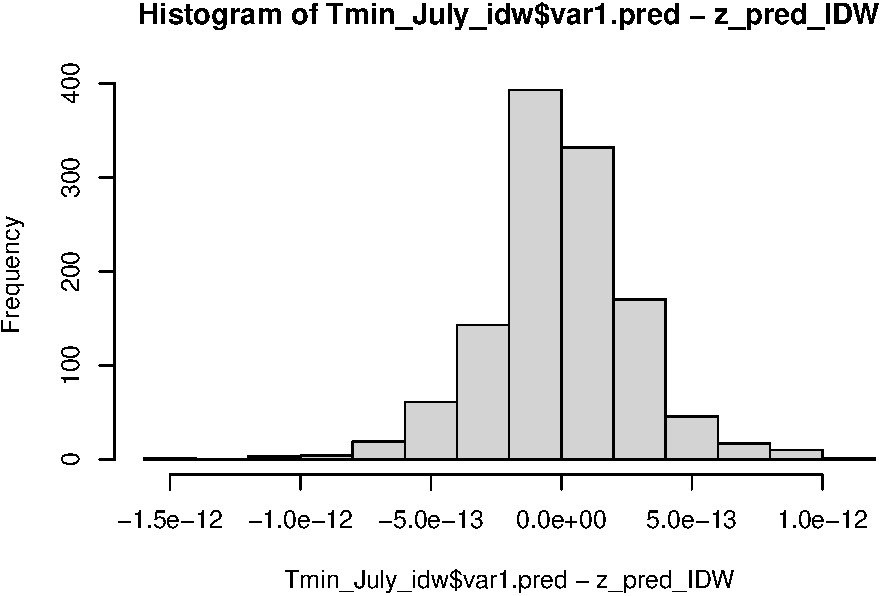
\includegraphics[width=0.25\linewidth]{fe_stat566_bak_files/figure-latex/unnamed-chunk-23-1}
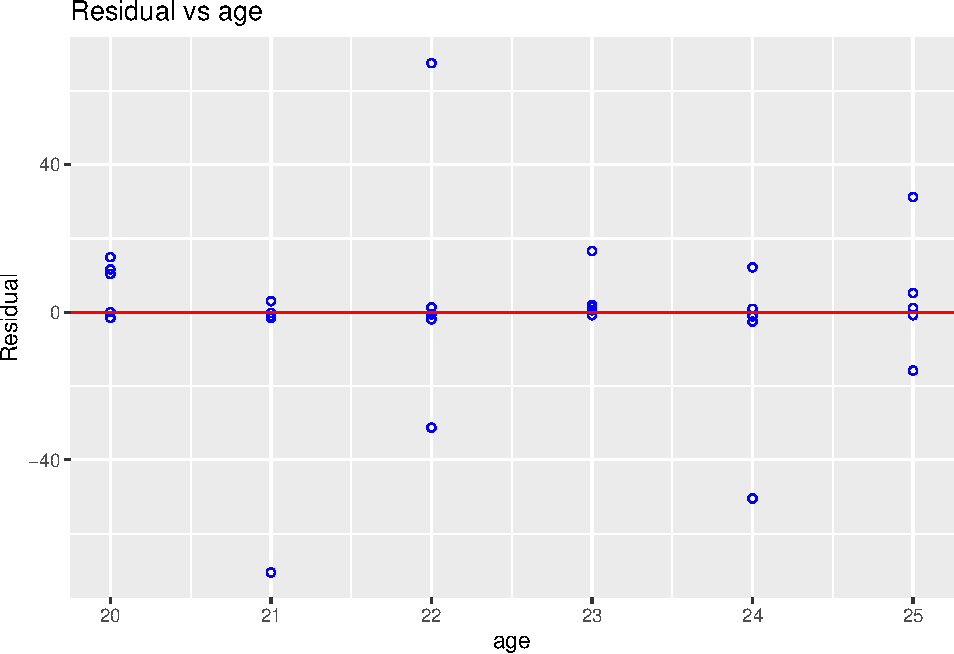
\includegraphics[width=0.25\linewidth]{fe_stat566_bak_files/figure-latex/unnamed-chunk-23-2}
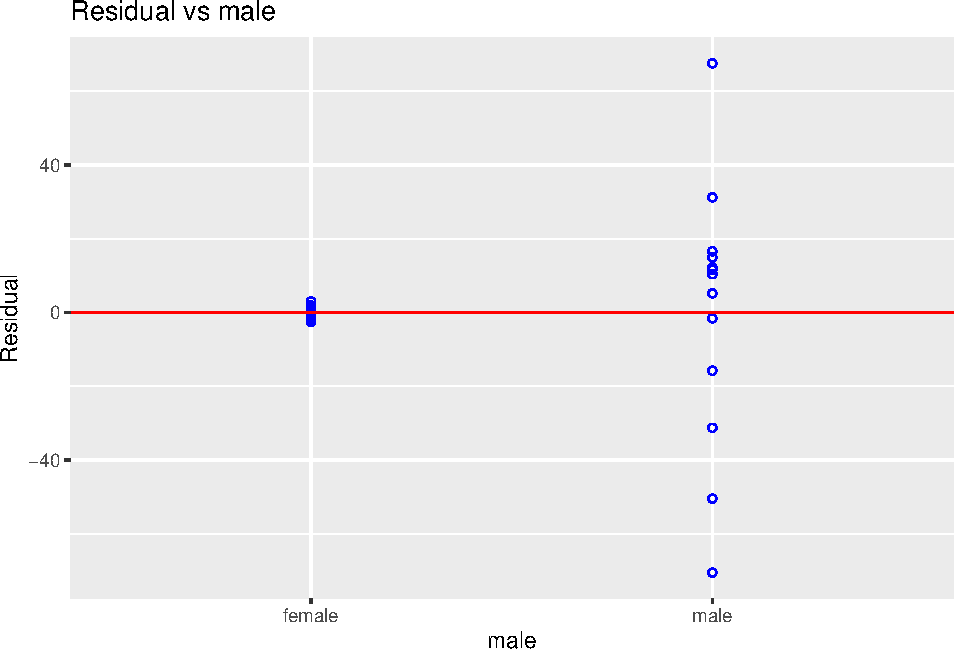
\includegraphics[width=0.25\linewidth]{fe_stat566_bak_files/figure-latex/unnamed-chunk-23-3}
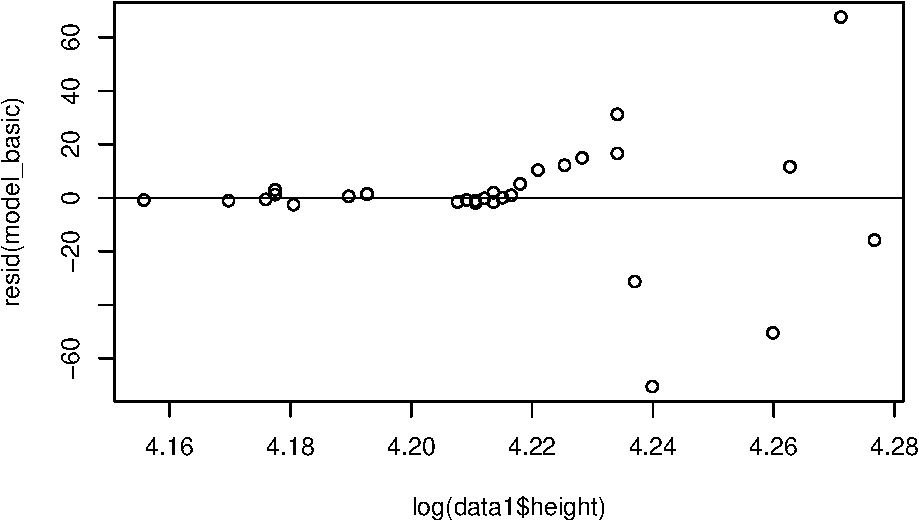
\includegraphics[width=0.25\linewidth]{fe_stat566_bak_files/figure-latex/unnamed-chunk-23-4}

In the plots of residuals versus predicted value of purity, there is no
significant pattern on this plot. Therefore, the fitted model is good
enough to describe the relationship between the mean value of focre and
the days, temperature, and fats.

The residuals in this plot are almost symmetrically distributed about
zero and hence zero mean assumption is not violated. Further, the
vertical deviation of the residuals from zero is about same for each
predicted value and hence the constant variance assumption is not
violated.

The points are along the straight line in the normal qq plot shown at
bottom left and the histogram of residuals shown at the top right is
about normal. These plots show no violation of normal distribution
assumption of residuals.

\begin{Shaded}
\begin{Highlighting}[]
\KeywordTok{favstats}\NormalTok{(force }\OperatorTok{~}\StringTok{ }\NormalTok{day, }\DataTypeTok{data =}\NormalTok{ fe_table_cookie)}
\KeywordTok{favstats}\NormalTok{(force }\OperatorTok{~}\StringTok{ }\NormalTok{fat, }\DataTypeTok{data =}\NormalTok{ fe_table_cookie)}
\KeywordTok{favstats}\NormalTok{(force }\OperatorTok{~}\StringTok{ }\NormalTok{temp, }\DataTypeTok{data =}\NormalTok{ fe_table_cookie)}
\KeywordTok{favstats}\NormalTok{(force }\OperatorTok{~}\StringTok{ }\NormalTok{day }\OperatorTok{+}\StringTok{ }\NormalTok{fat, }\DataTypeTok{data =}\NormalTok{ fe_table_cookie)}
\KeywordTok{favstats}\NormalTok{(force }\OperatorTok{~}\StringTok{ }\NormalTok{temp }\OperatorTok{+}\StringTok{ }\NormalTok{fat, }\DataTypeTok{data =}\NormalTok{ fe_table_cookie)}
\KeywordTok{favstats}\NormalTok{(force }\OperatorTok{~}\StringTok{ }\NormalTok{temp }\OperatorTok{+}\StringTok{ }\NormalTok{day, }\DataTypeTok{data =}\NormalTok{ fe_table_cookie)}

\NormalTok{fe_table_cookie}\OperatorTok{$}\NormalTok{day_r <-}\StringTok{ }\KeywordTok{as.random}\NormalTok{(fe_table_cookie}\OperatorTok{$}\NormalTok{day)}
\NormalTok{fe_table_cookie}\OperatorTok{$}\NormalTok{temp_f <-}\StringTok{ }\KeywordTok{as.fixed}\NormalTok{(fe_table_cookie}\OperatorTok{$}\NormalTok{temp)}
\NormalTok{fe_table_cookie}\OperatorTok{$}\NormalTok{fat_f <-}\StringTok{ }\KeywordTok{as.fixed}\NormalTok{(fe_table_cookie}\OperatorTok{$}\NormalTok{fat)}
\NormalTok{fe_model_cookie1 <-}\StringTok{ }\KeywordTok{aov}\NormalTok{(}\DataTypeTok{formula =}\NormalTok{ force }\OperatorTok{~}\StringTok{ }\NormalTok{day_r }\OperatorTok{+}\StringTok{ }\NormalTok{fat_f }\OperatorTok{+}\StringTok{ }\NormalTok{fat_f }\OperatorTok\StringTok{ }\NormalTok{day_r }\OperatorTok{+}\StringTok{ }
\StringTok{    }\NormalTok{temp_f }\OperatorTok\StringTok{ }\NormalTok{day_r }\OperatorTok{+}\StringTok{ }\NormalTok{temp_f }\OperatorTok{+}\StringTok{ }\NormalTok{temp_f}\OperatorTok{:}\NormalTok{fat_f, }\DataTypeTok{data =}\NormalTok{ fe_table_cookie)}
\KeywordTok{gad}\NormalTok{(fe_model_cookie1)}

\NormalTok{fe_model_cookie2 <-}\StringTok{ }\KeywordTok{lmer}\NormalTok{(}\DataTypeTok{formula =}\NormalTok{ force }\OperatorTok{~}\StringTok{ }\NormalTok{(}\DecValTok{1} \OperatorTok{|}\StringTok{ }\NormalTok{day) }\OperatorTok{+}\StringTok{ }\NormalTok{fat }\OperatorTok{+}\StringTok{ }\NormalTok{(}\DecValTok{1} \OperatorTok{|}\StringTok{ }\NormalTok{day}\OperatorTok{:}\NormalTok{fat) }\OperatorTok{+}\StringTok{ }
\StringTok{    }\NormalTok{temp }\OperatorTok{+}\StringTok{ }\NormalTok{(}\DecValTok{1} \OperatorTok{|}\StringTok{ }\NormalTok{day}\OperatorTok{:}\NormalTok{temp) }\OperatorTok{+}\StringTok{ }\NormalTok{temp}\OperatorTok{:}\NormalTok{fat, }\DataTypeTok{data =}\NormalTok{ fe_table_cookie, }\DataTypeTok{REML =} \OtherTok{TRUE}\NormalTok{)}
\KeywordTok{summary}\NormalTok{(fe_model_cookie2)}
\KeywordTok{confint}\NormalTok{(fe_model_cookie2)}

\NormalTok{fe_model_cookie3 <-}\StringTok{ }\KeywordTok{aov}\NormalTok{(}\DataTypeTok{formula =}\NormalTok{ force }\OperatorTok{~}\StringTok{ }\NormalTok{day_r }\OperatorTok{+}\StringTok{ }\NormalTok{fat_f }\OperatorTok{+}\StringTok{ }\NormalTok{temp_f }\OperatorTok{+}\StringTok{ }\NormalTok{temp_f }\OperatorTok\StringTok{ }
\StringTok{    }\NormalTok{day_r }\OperatorTok{+}\StringTok{ }\NormalTok{temp_f}\OperatorTok{:}\NormalTok{fat_f, }\DataTypeTok{data =}\NormalTok{ fe_table_cookie)}
\KeywordTok{gad}\NormalTok{(fe_model_cookie3)}
\NormalTok{fe_model_cookie4 <-}\StringTok{ }\KeywordTok{lmer}\NormalTok{(}\DataTypeTok{formula =}\NormalTok{ force }\OperatorTok{~}\StringTok{ }\NormalTok{(}\DecValTok{1} \OperatorTok{|}\StringTok{ }\NormalTok{day) }\OperatorTok{+}\StringTok{ }\NormalTok{fat }\OperatorTok{+}\StringTok{ }\NormalTok{temp }\OperatorTok{+}\StringTok{ }\NormalTok{(}\DecValTok{1} \OperatorTok{|}\StringTok{ }\NormalTok{day}\OperatorTok{:}\NormalTok{temp) }\OperatorTok{+}\StringTok{ }
\StringTok{    }\NormalTok{temp }\OperatorTok{*}\StringTok{ }\NormalTok{fat, }\DataTypeTok{data =}\NormalTok{ fe_table_cookie, }\DataTypeTok{REML =} \OtherTok{TRUE}\NormalTok{)}
\KeywordTok{summary}\NormalTok{(fe_model_cookie4)}
\KeywordTok{confint}\NormalTok{(fe_model_cookie4)}

\NormalTok{temp_fat <-}\StringTok{ }\KeywordTok{pairs}\NormalTok{(}\KeywordTok{lsmeans}\NormalTok{(fe_model_cookie4, }\OperatorTok{~}\NormalTok{temp }\OperatorTok{|}\StringTok{ }\NormalTok{fat))}
\NormalTok{fat_temp <-}\StringTok{ }\KeywordTok{pairs}\NormalTok{(}\KeywordTok{lsmeans}\NormalTok{(fe_model_cookie4, }\OperatorTok{~}\NormalTok{fat }\OperatorTok{|}\StringTok{ }\NormalTok{temp))}
\KeywordTok{test}\NormalTok{(}\KeywordTok{rbind}\NormalTok{(temp_fat, fat_temp), }\DataTypeTok{adjust =} \StringTok{"tukey"}\NormalTok{)}
\NormalTok{temp_day <-}\StringTok{ }\KeywordTok{pairs}\NormalTok{(}\KeywordTok{lsmeans}\NormalTok{(fe_model_cookie3, }\OperatorTok{~}\NormalTok{temp_f }\OperatorTok{|}\StringTok{ }\NormalTok{day_r))}
\NormalTok{day_temp <-}\StringTok{ }\KeywordTok{pairs}\NormalTok{(}\KeywordTok{lsmeans}\NormalTok{(fe_model_cookie3, }\OperatorTok{~}\NormalTok{day_r }\OperatorTok{|}\StringTok{ }\NormalTok{temp_f))}
\KeywordTok{test}\NormalTok{(}\KeywordTok{rbind}\NormalTok{(temp_day, day_temp), }\DataTypeTok{adjust =} \StringTok{"tukey"}\NormalTok{)}

\NormalTok{fe_residual_cookie <-}\StringTok{ }\KeywordTok{rstudent}\NormalTok{(fe_model_cookie4)}
\KeywordTok{plot}\NormalTok{(fe_residual_cookie)}
\KeywordTok{plot}\NormalTok{(fe_model_cookie4)}
\KeywordTok{qqnorm}\NormalTok{(fe_residual_cookie)}
\KeywordTok{qqline}\NormalTok{(fe_residual_cookie)}
\KeywordTok{hist}\NormalTok{(fe_residual_cookie)}
\end{Highlighting}
\end{Shaded}


\end{document}
